\section{Validierungstests und Ergebnisse}
\subsection{Zielsetzung der Validierung}
Ziel der Validierung war es, zu überprüfen, ob die definierten Toleranzanforderungen eingehalten werden können und ob alle eingesetzten Aktoren und Sensoren wie vorgesehen funktionieren. Der Schwerpunkt lag dabei auf der grundsätzlichen Funktionsfähigkeit der einzelnen Komponenten sowie auf der Bewertung der erreichbaren Positioniergenauigkeit.

Die durchgeführten Tests stellen keine vollständige Serien- oder Langzeitvalidierung dar, sondern dienen als funktionale Überprüfung des Systems im Prototypenstadium. Das Ziel war es, eine belastbare Grundlage für die weitere Integration und den späteren automatisierten Betrieb zu schaffen.

\subsection{Validierungsstrategie und Vorgehensweise}
Die Validierung wurde ausschließlich über manuelle Einzeltests durchgeführt. Dabei wurden alle Komponenten separat betrachtet, um deren Funktion unabhängig voneinander bewerten zu können. Eine automatisierte Ablaufsteuerung wurde bewusst nicht eingesetzt.

Die Linearachsen wurden zunächst einzeln getestet. Nach einer Referenzfahrt wurden definierte Positionen innerhalb des Verfahrbereichs mehrfach angefahren. Anschließend wurde eine Kombination mehrerer Achsbewegungen durchgeführt, bei der eine Achse auf eine feste Position verfahren wurde, danach eine zweite Achse bewegt und anschließend wieder zur ursprünglichen Position zurückgefahren wurde. Dieser Ablauf wurde mehrfach wiederholt, um die Wiederholgenauigkeit zu überprüfen. Die resultierenden Positionen wurden mit einer Messuhr kontrolliert.

Zusätzlich wurden digitale Ein- und Ausgangssignale geprüft, indem Aktoren gezielt angesteuert und die zugehörigen Sensorsignale ausgewertet wurden.

\subsection{Eingesetzte Werkzeuge}
Für die Validierung kamen folgende Werkzeuge zum Einsatz:

\begin{itemize}
    \item TMCL-IDE Version 3.9.0 zur Ansteuerung und Überwachung des TMCM-6110
    \item WAGO-Steuerung, getestet über ein einfaches Python-Programm zum Auslesen von Eingängen und Setzen von Ausgängen
    \item Messuhr (\qty{2}{\micro\metre} Auflösung) zur Überprüfung der Positioniergenauigkeit der Linearachsen
    \item PC zur Bedienung der Software und zur Visualisierung der Signale
\end{itemize}

Die im Rahmen der Validierung eingesetzten Testskripte zur Ansteuerung des
TMCM-6110 sowie der WAGO-Steuerung sind aus Gründen der Übersichtlichkeit
im Anhang aufgeführt (Code-Ausschnitt~\ref{lst:gui_py} bis~\ref{lst:tmcl_test}).

\subsection{Durchgeführte Tests mit dem TMCM-6110}
\subsubsection{Tests der Linearachsen}
Die Linearachsen in X-, Y- und Z-Richtung wurden einzeln getestet. Nach der jeweiligen Referenzfahrt wurden definierte Positionen innerhalb des Verfahrbereichs mehrfach angefahren. Zusätzlich wurden die Endlagen gezielt angefahren, um die Funktion der Endlagensensorik zu überprüfen.

Zur Bewertung der Wiederholgenauigkeit wurde jede Achse mehrmals zwischen festgelegten Positionen verfahren. Die Positionsabweichung wurde dabei mit einer Messuhr erfasst. Während der Tests traten keine Schrittverluste auf. Zudem waren keine auffälligen Geräusche oder unruhigen Bewegungen feststellbar.

Die Messergebnisse zeigten eine stabile Wiederholgenauigkeit. Die gemessene Abweichung lag bei maximal \qty{8}{\micro\metre} für die X-Achse, bei maximal \qty{4}{\micro\metre} für die Y-Achse und bei maximal \qty{6}{\micro\metre} für die Z-Achse. Damit liegen die erzielten Werte innerhalb der im Rahmen der Anforderungsanalyse definierten Toleranzen.

\begin{figure}[H]
    \centering
    \begin{subfigure}[t]{0.45\textwidth}
        \centering
        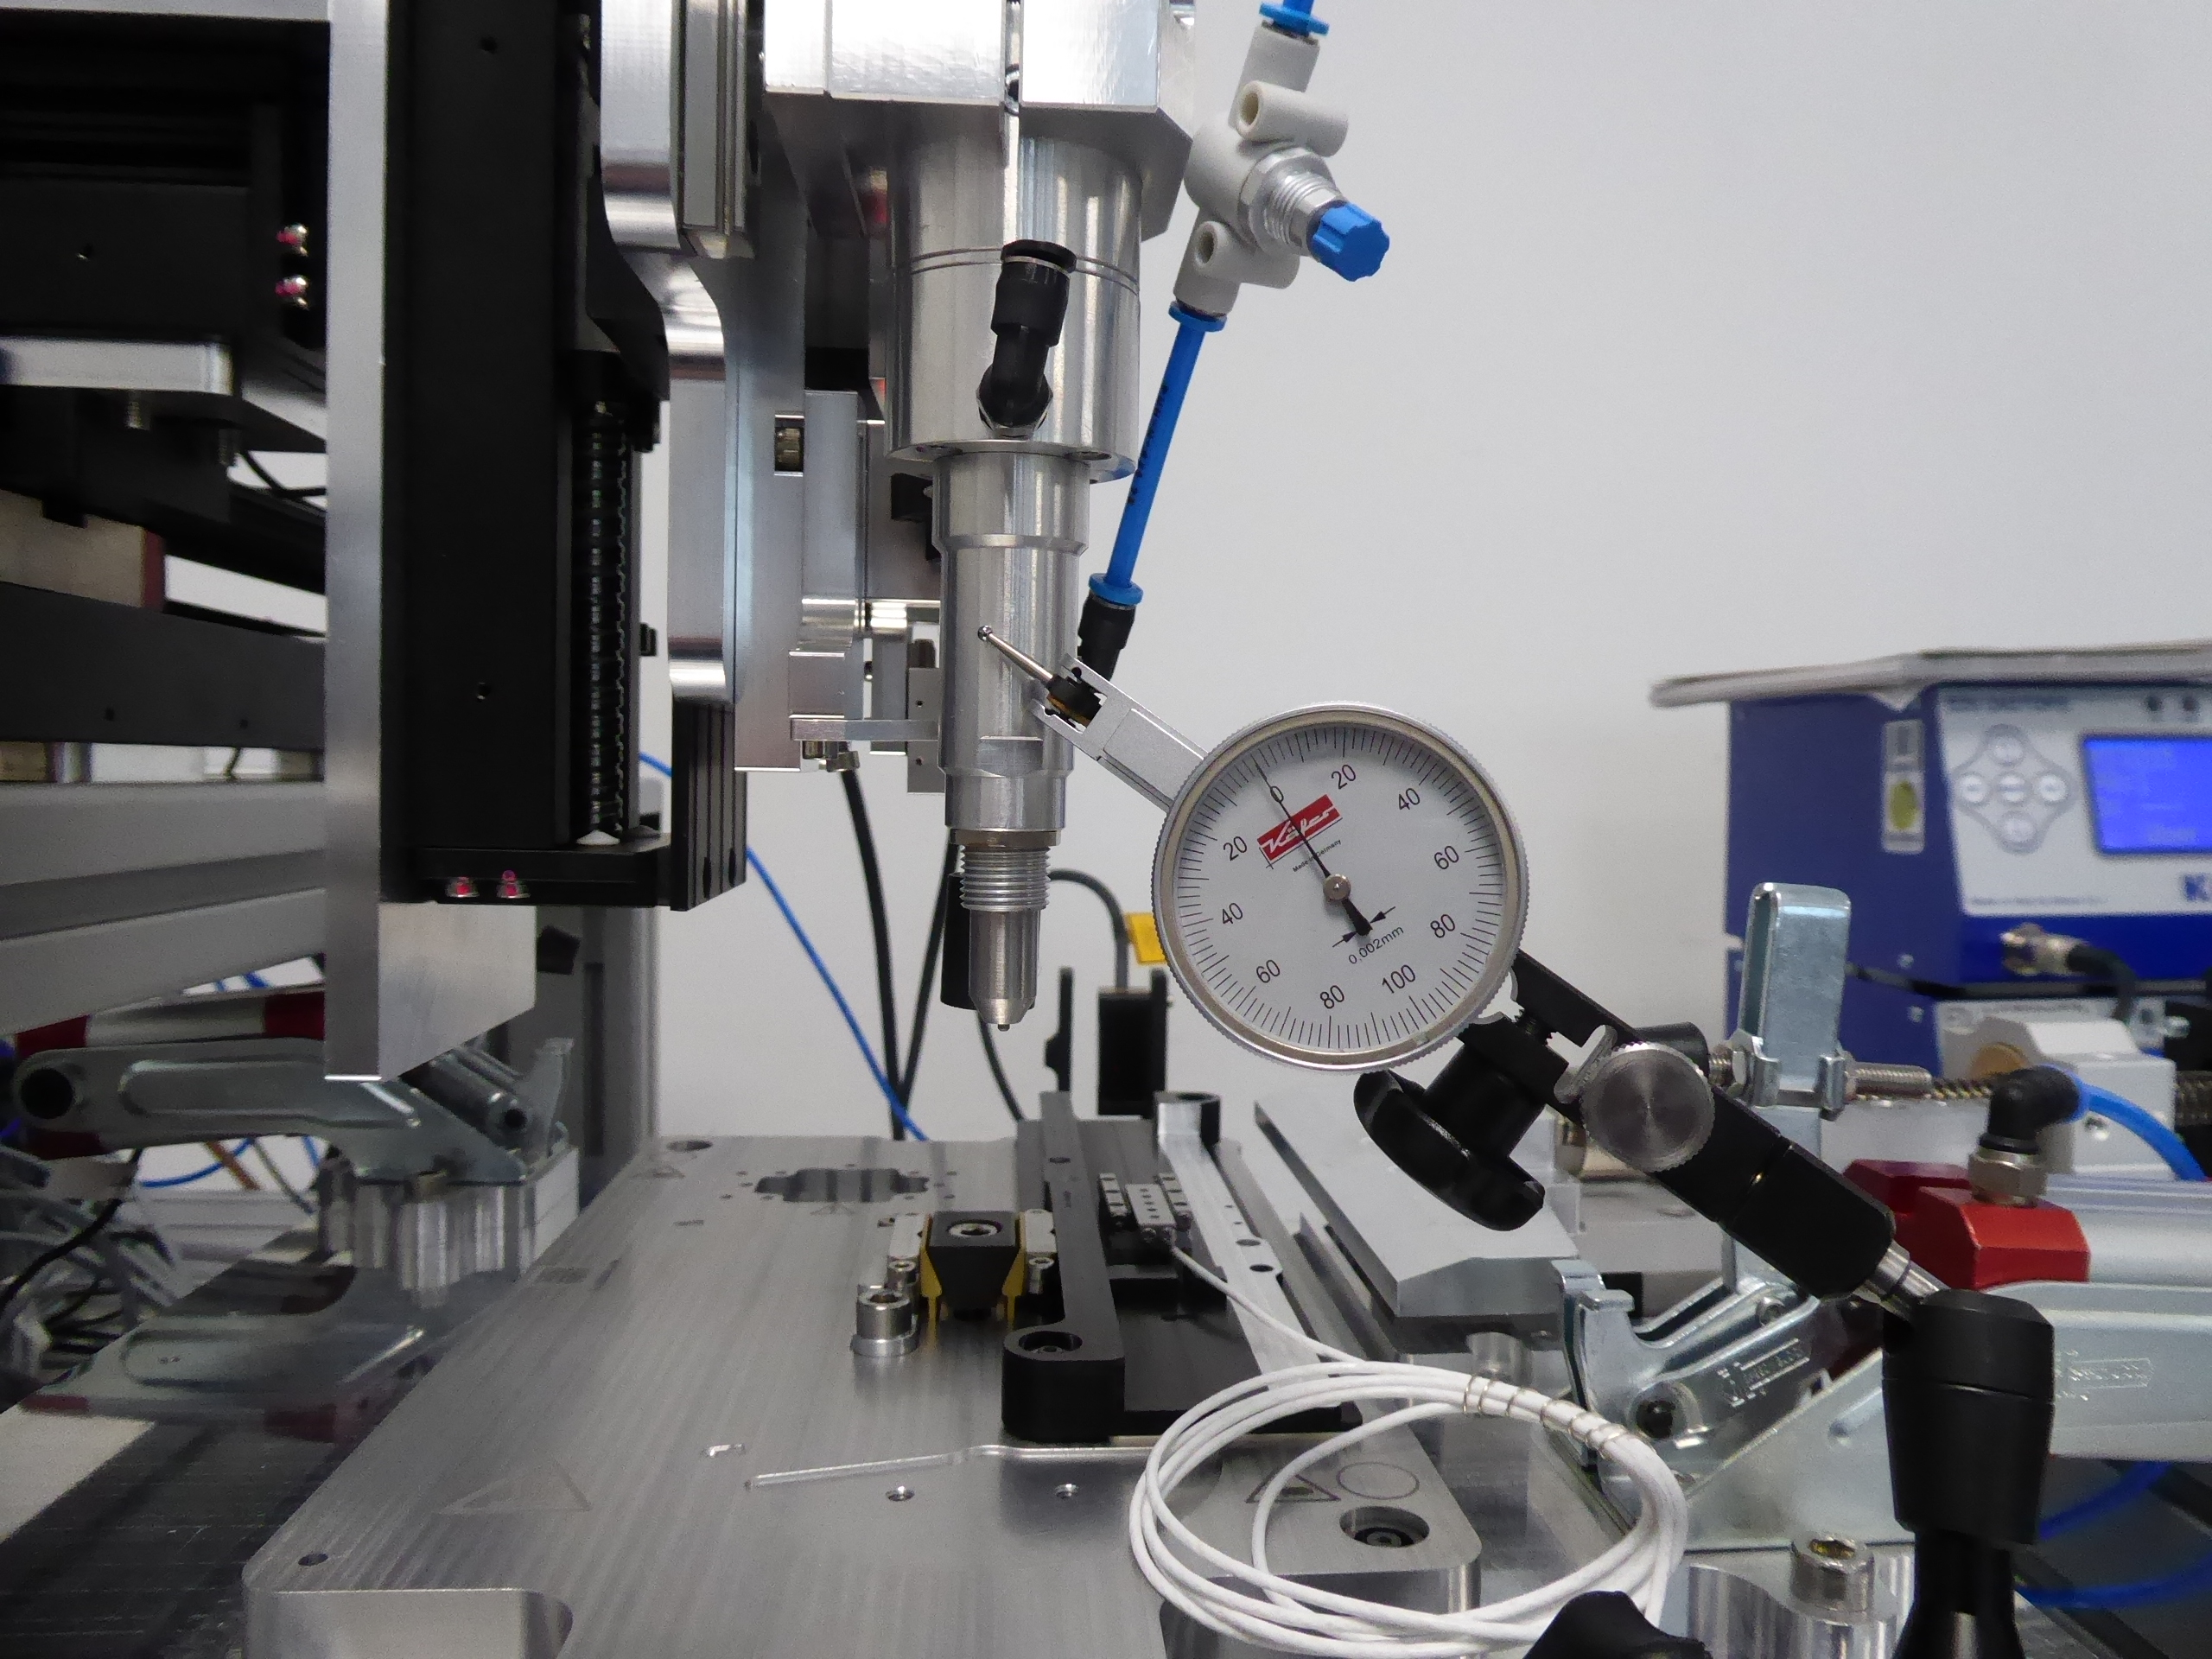
\includegraphics[width=\textwidth]{Bilder/06_Ergebnisse/x_start.JPG}
        \caption{Startposition der X-Achse}
        \label{fig:x_start}
    \end{subfigure}
    \hfill
    \begin{subfigure}[t]{0.45\textwidth}
        \centering
        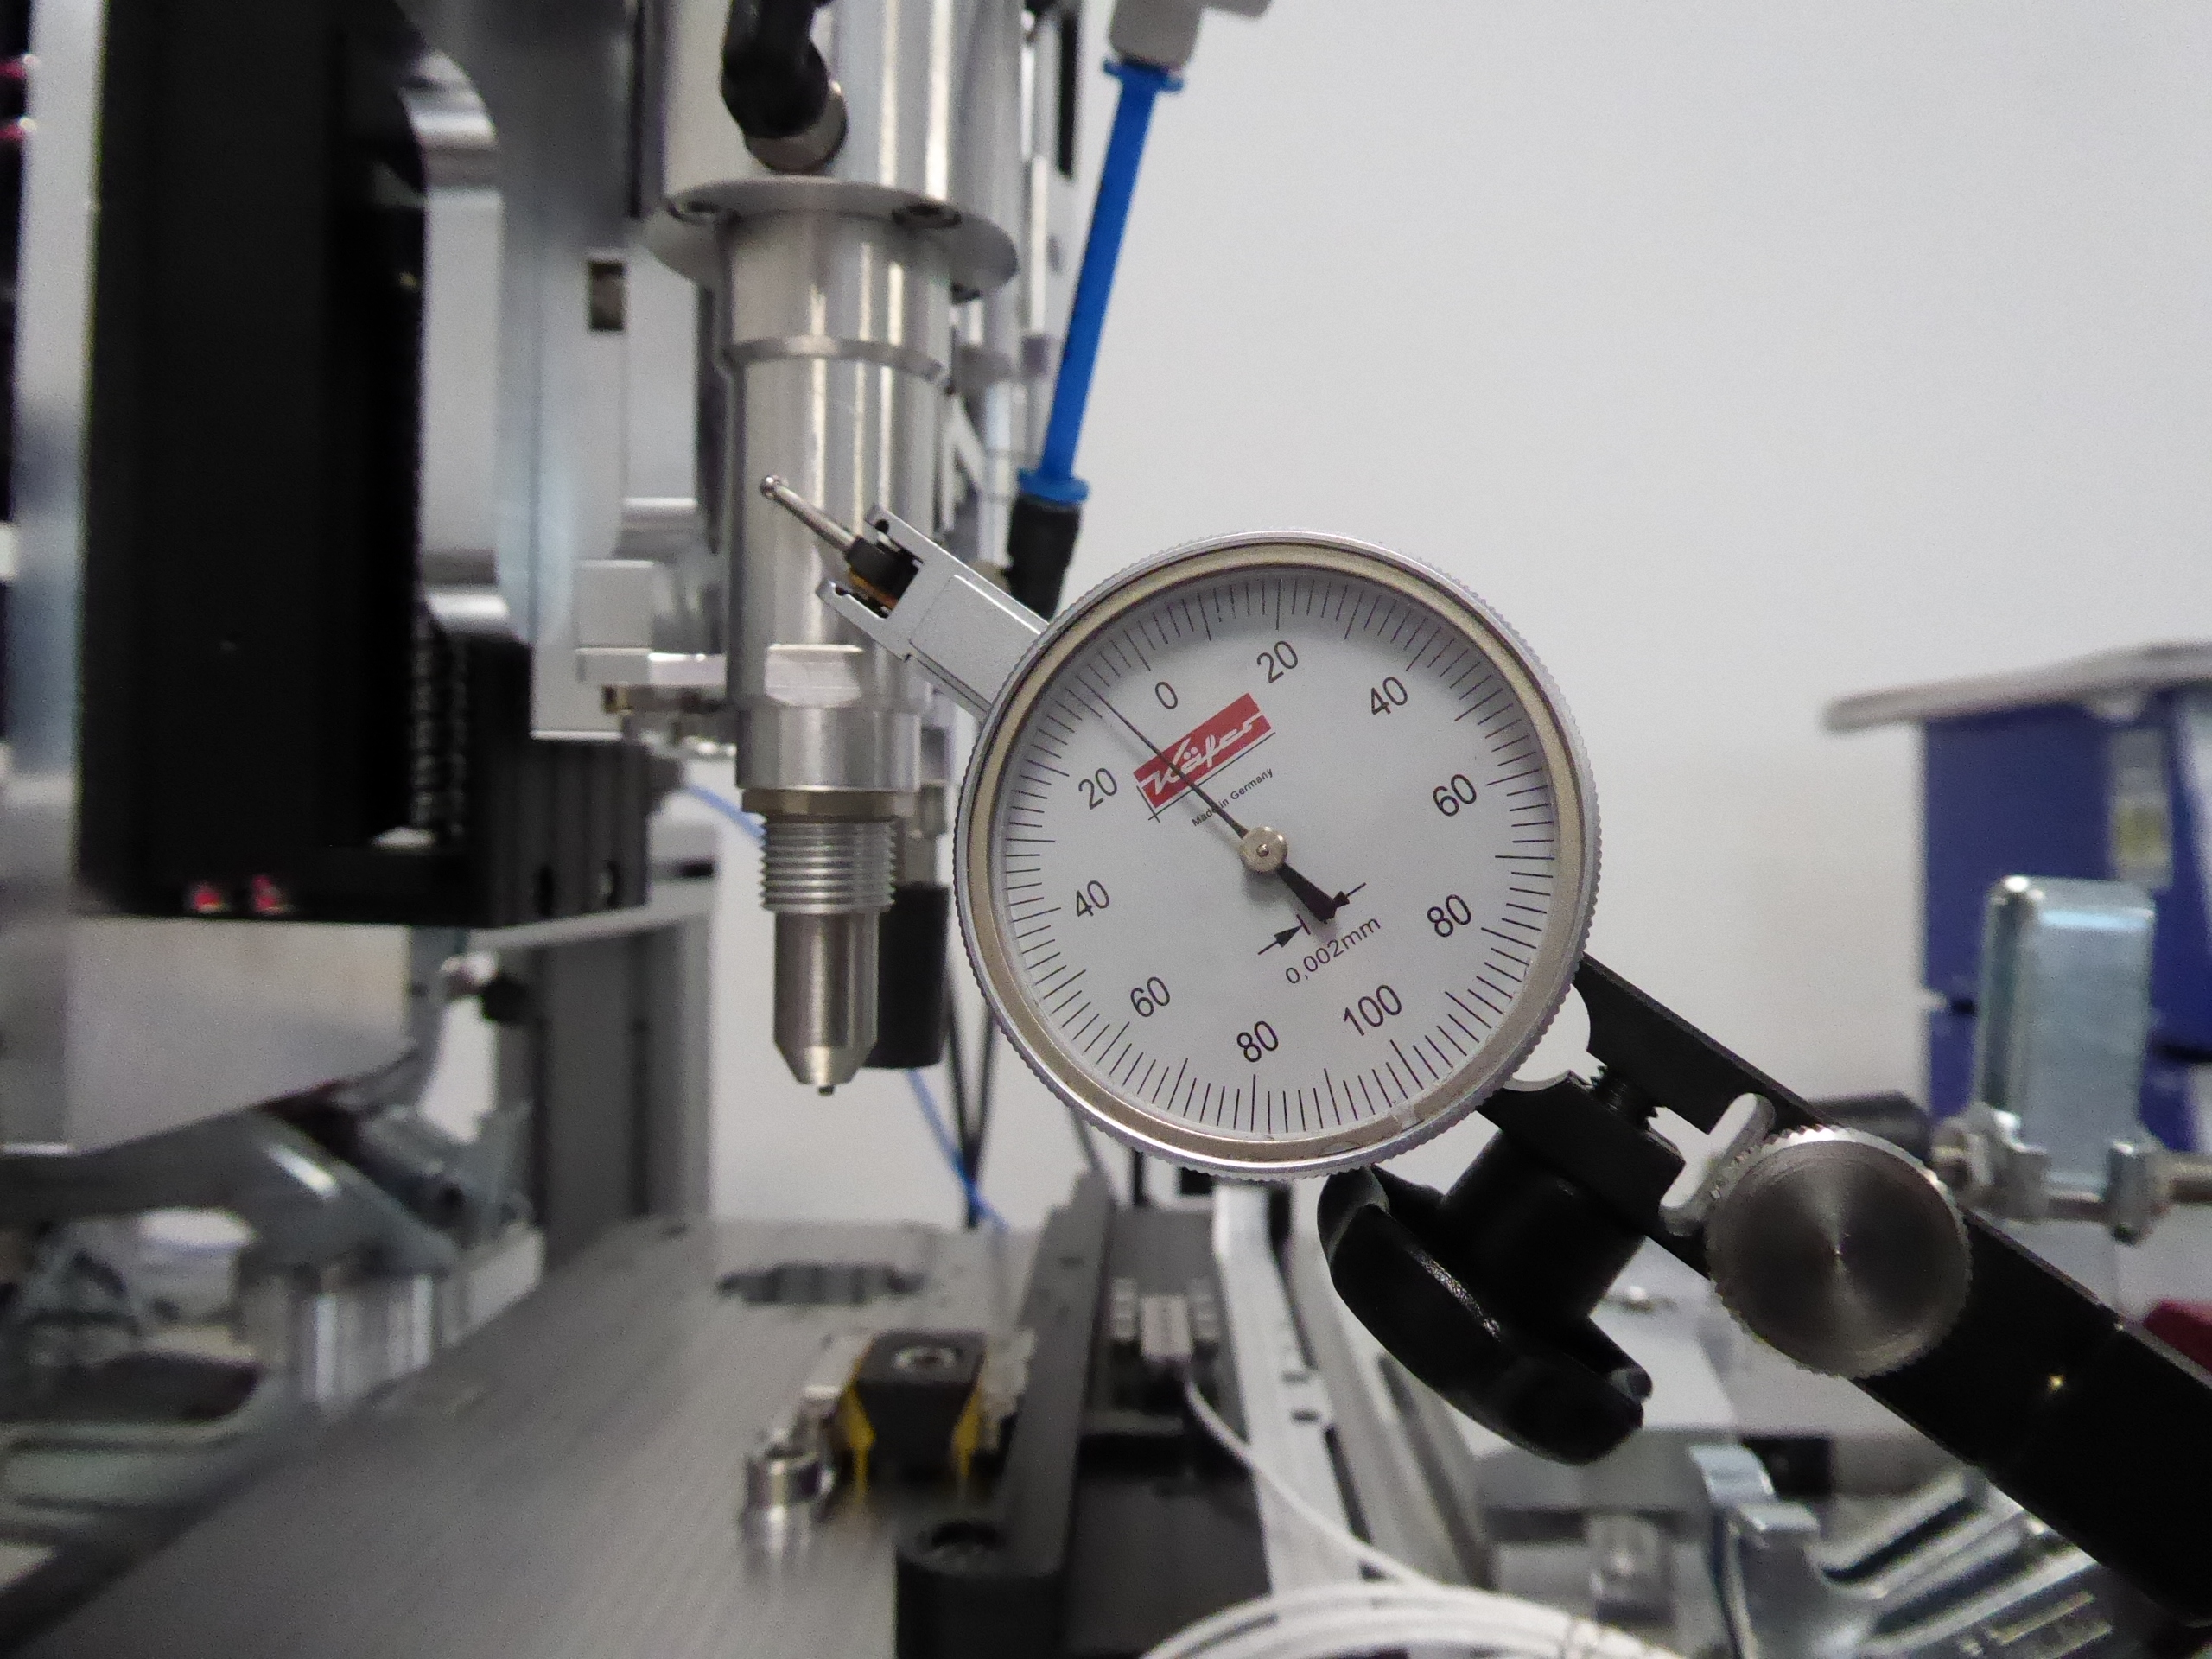
\includegraphics[width=\textwidth]{Bilder/06_Ergebnisse/x_end.JPG}
        \caption{Endposition der X-Achse}
        \label{fig:x_ende}
    \end{subfigure}

    \caption{Messaufbau zur Überprüfung der Wiederholgenauigkeit der X-Achse}
    \label{fig:x_achse_messung}
\end{figure}

\begin{figure}[H]
    \centering
    \begin{subfigure}[t]{0.45\textwidth}
        \centering
        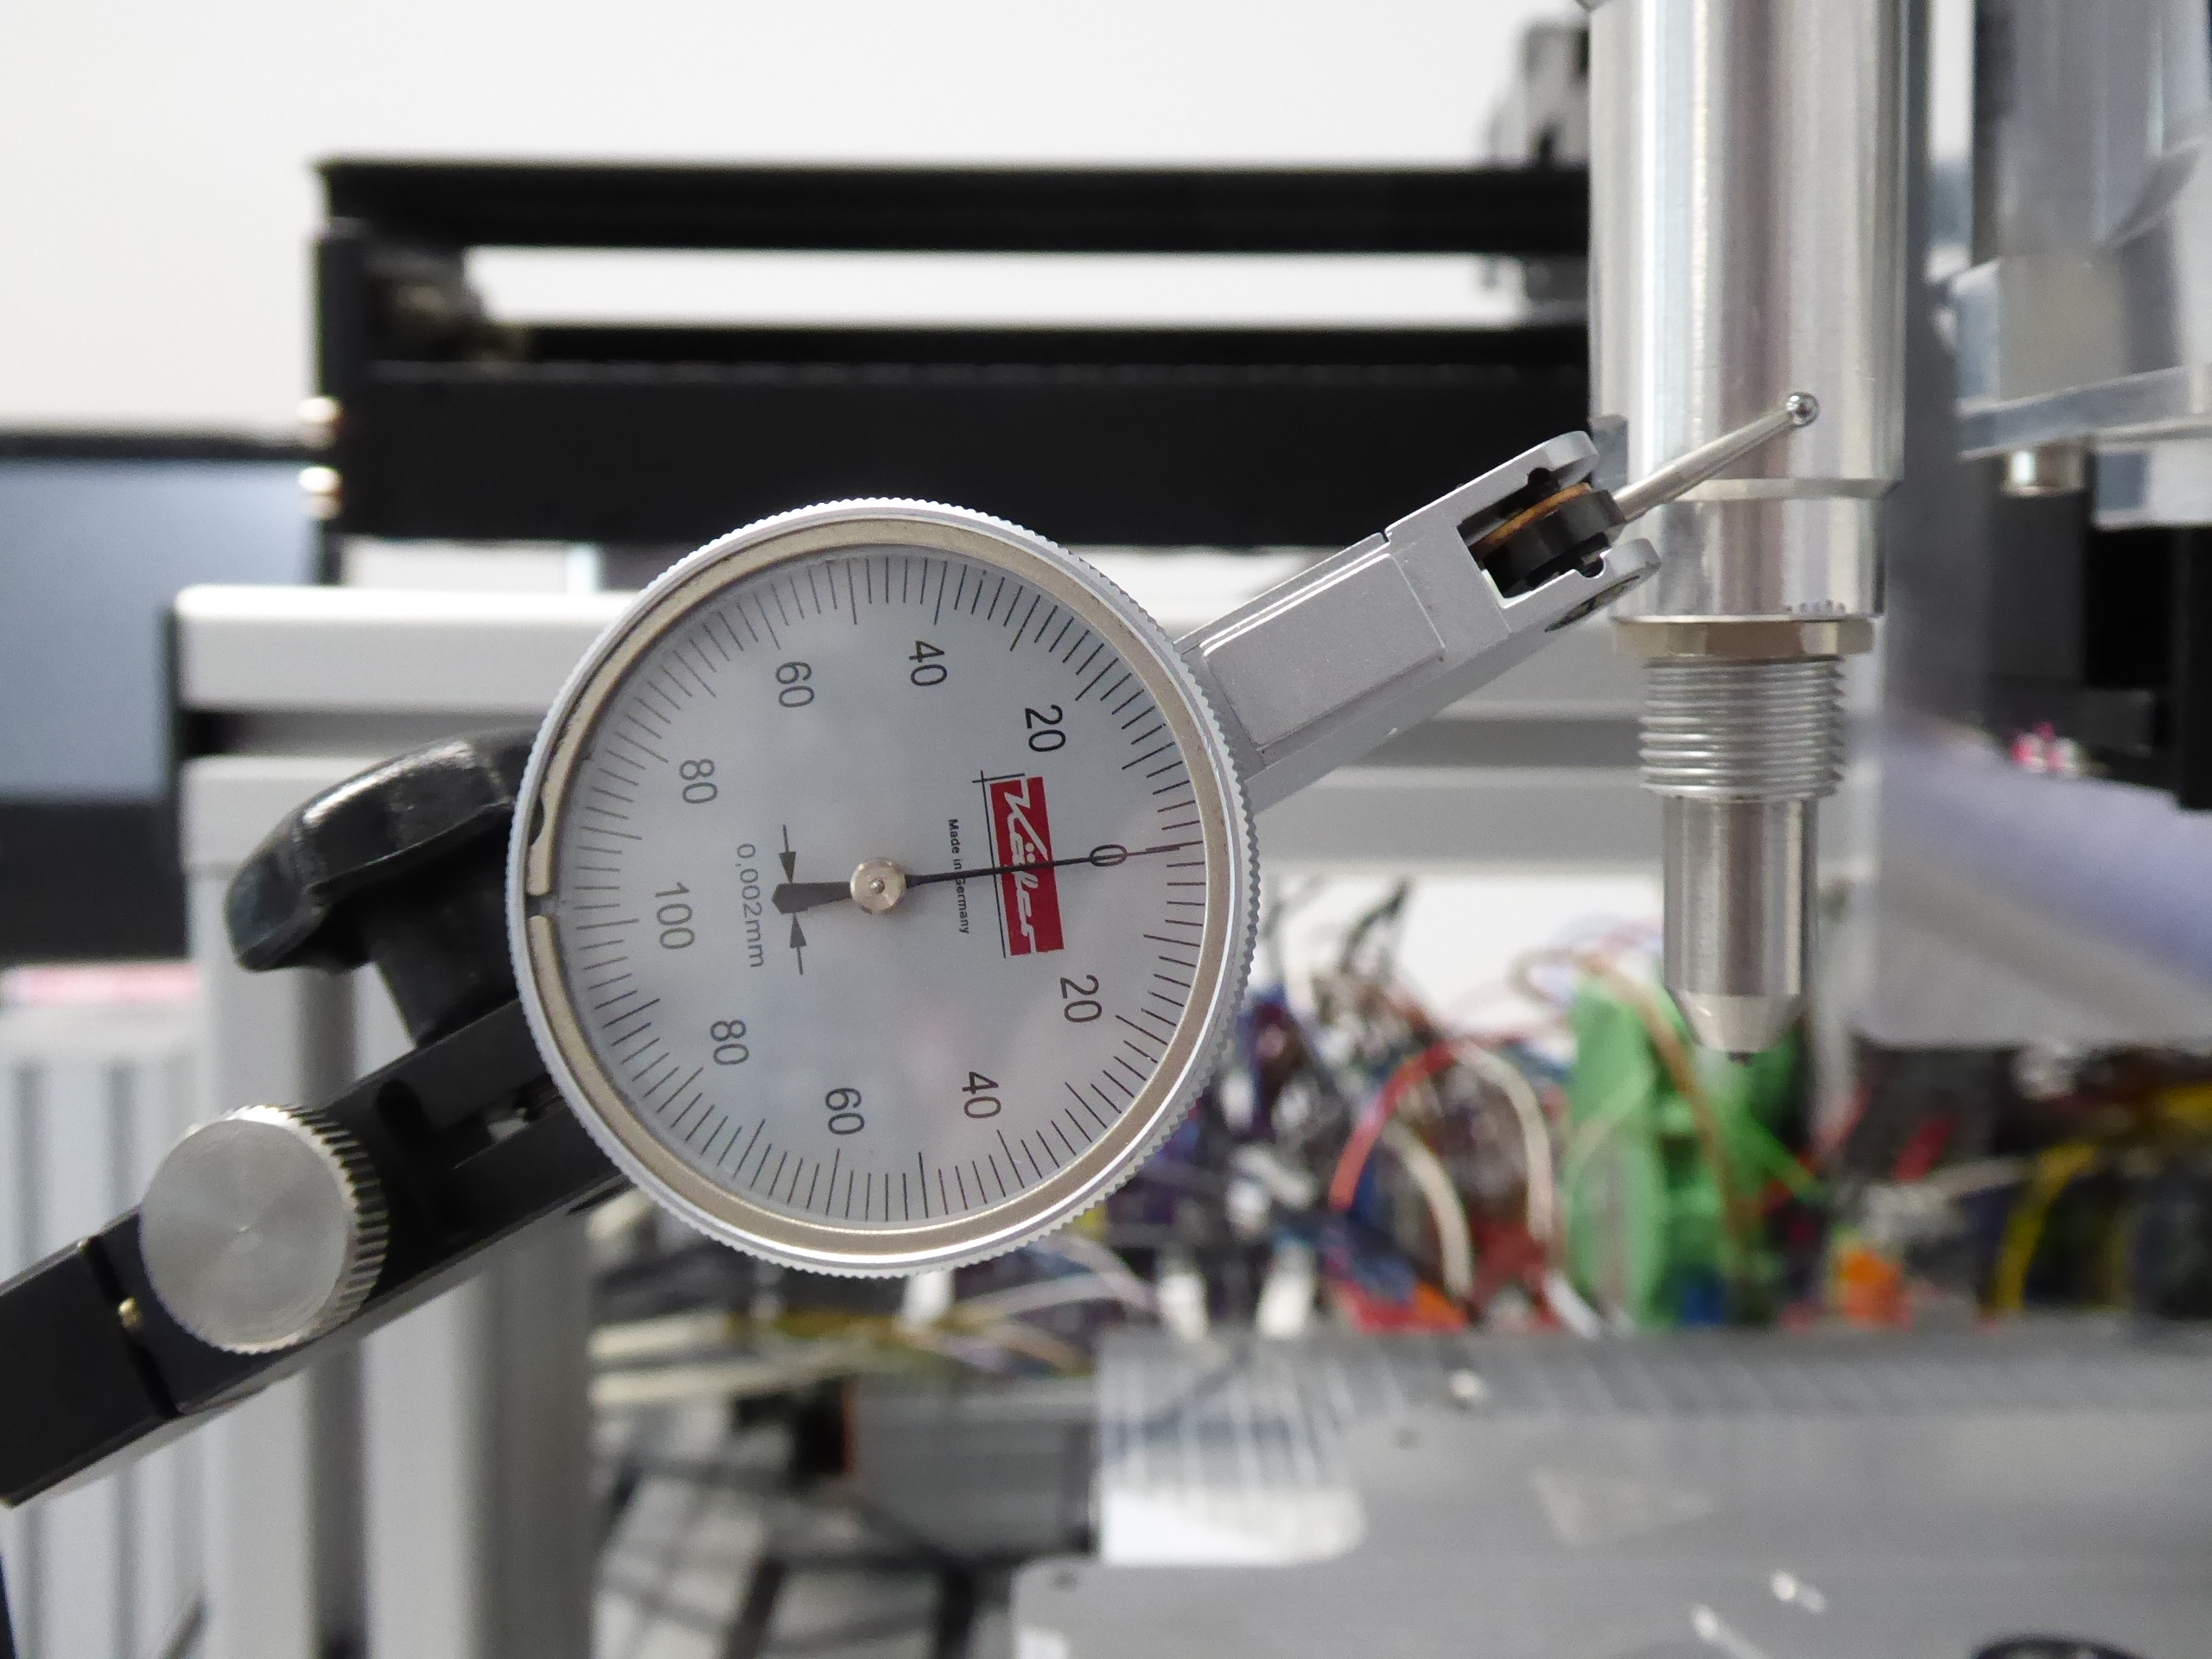
\includegraphics[width=\textwidth]{Bilder/06_Ergebnisse/y_start.JPG}
        \caption{Startposition der Y-Achse}
    \end{subfigure}
    \hfill
    \begin{subfigure}[t]{0.45\textwidth}
        \centering
        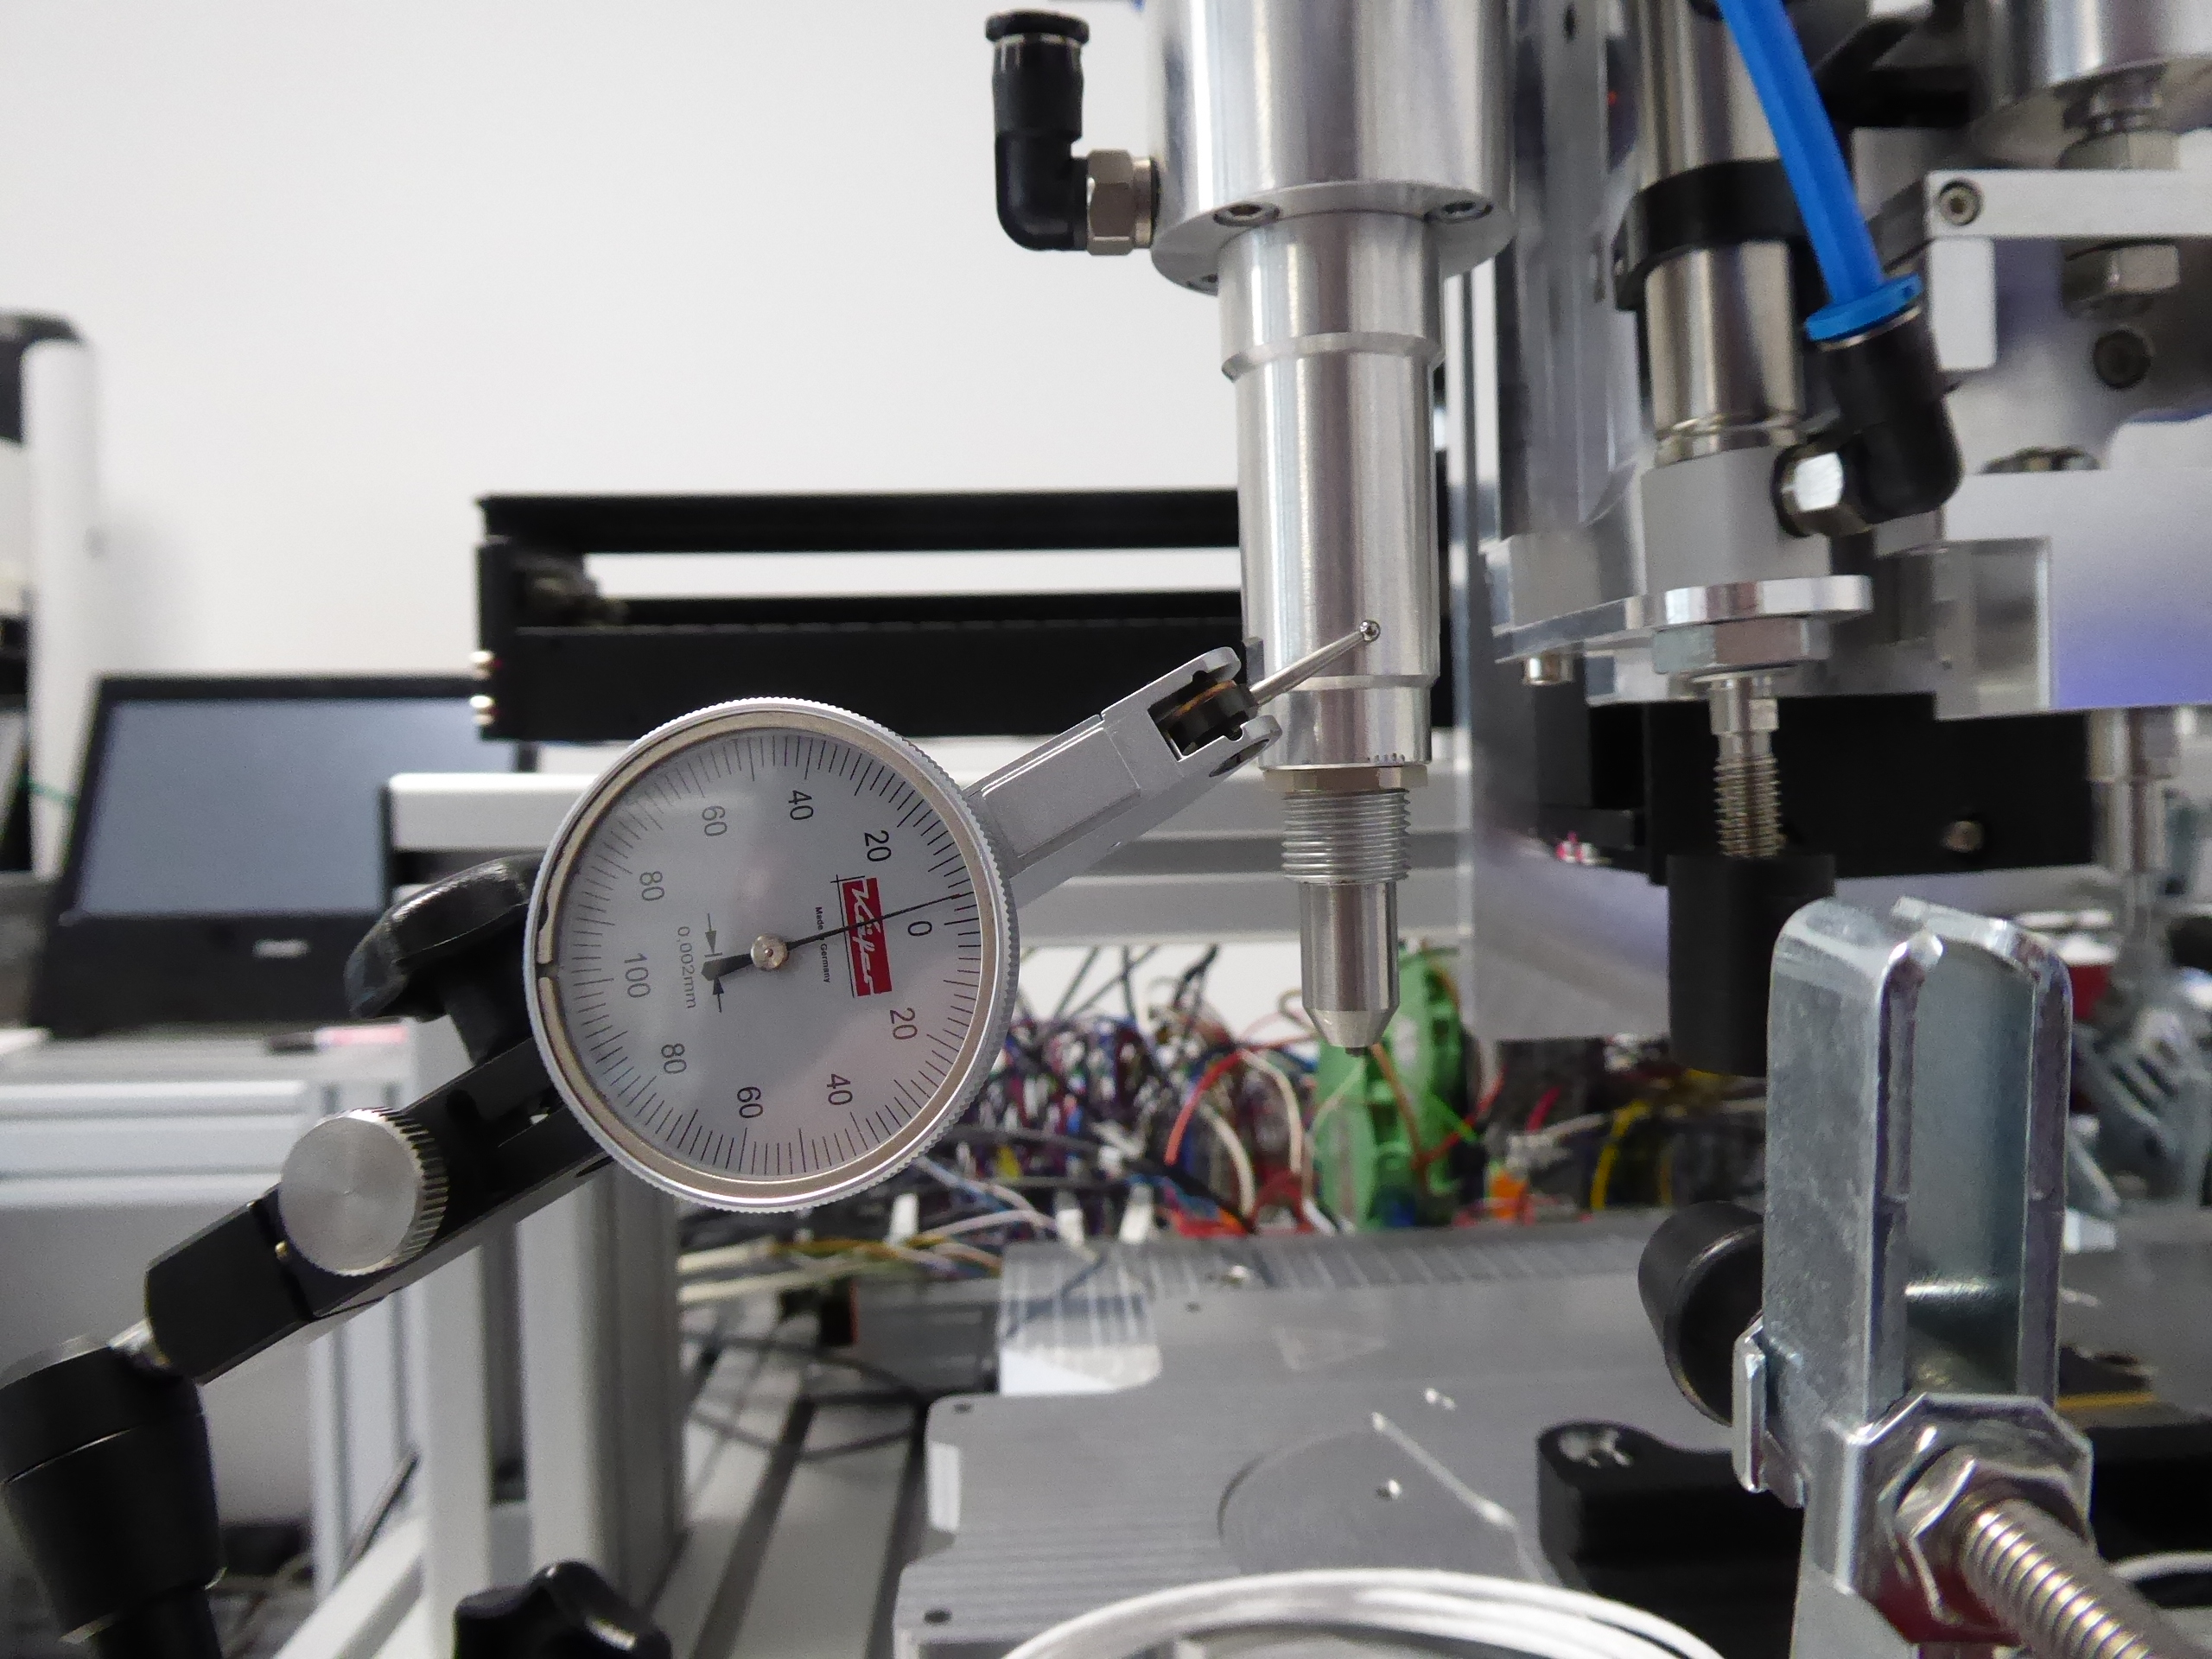
\includegraphics[width=\textwidth]{Bilder/06_Ergebnisse/y_end.JPG}
        \caption{Endposition der Y-Achse}
    \end{subfigure}

    \caption{Messaufbau zur Überprüfung der Wiederholgenauigkeit der Y-Achse}
    \label{fig:y_achse_messung}
\end{figure}

\begin{figure}[H]
    \centering
    \begin{subfigure}[t]{0.45\textwidth}
        \centering
        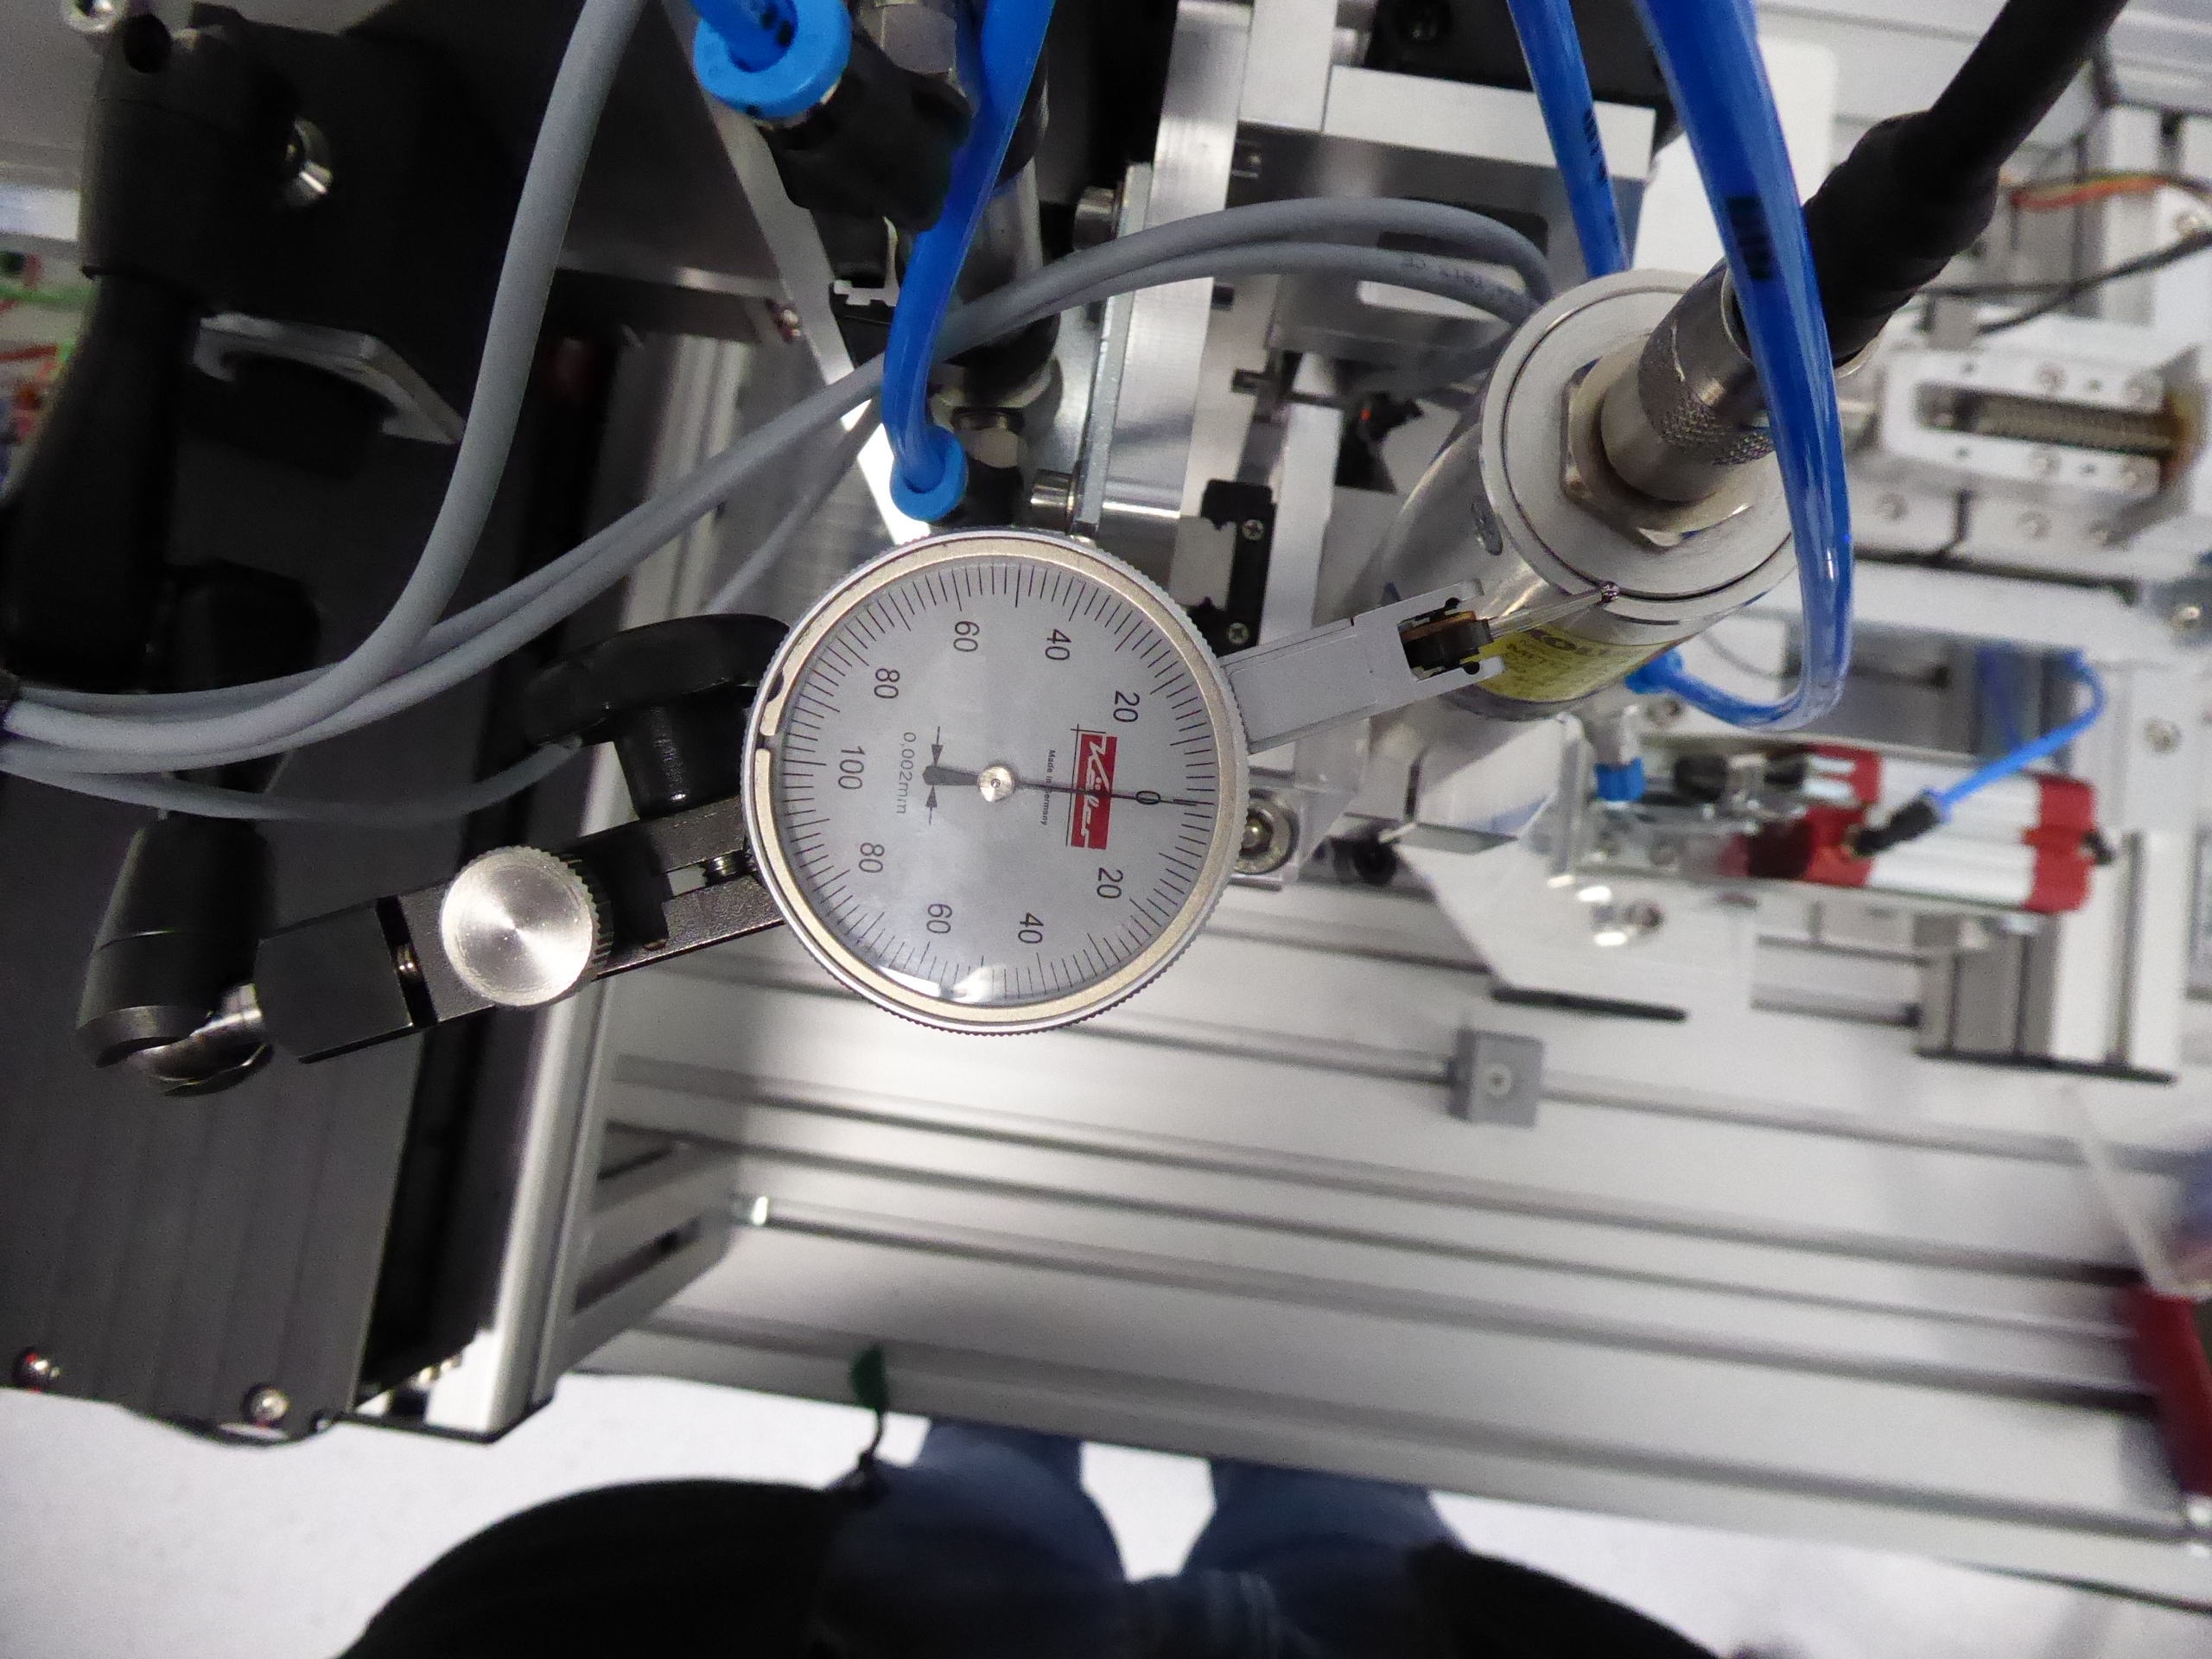
\includegraphics[width=\textwidth]{Bilder/06_Ergebnisse/z_start.JPG}
        \caption{Startposition der Z-Achse}
    \end{subfigure}
    \hfill
    \begin{subfigure}[t]{0.45\textwidth}
        \centering
        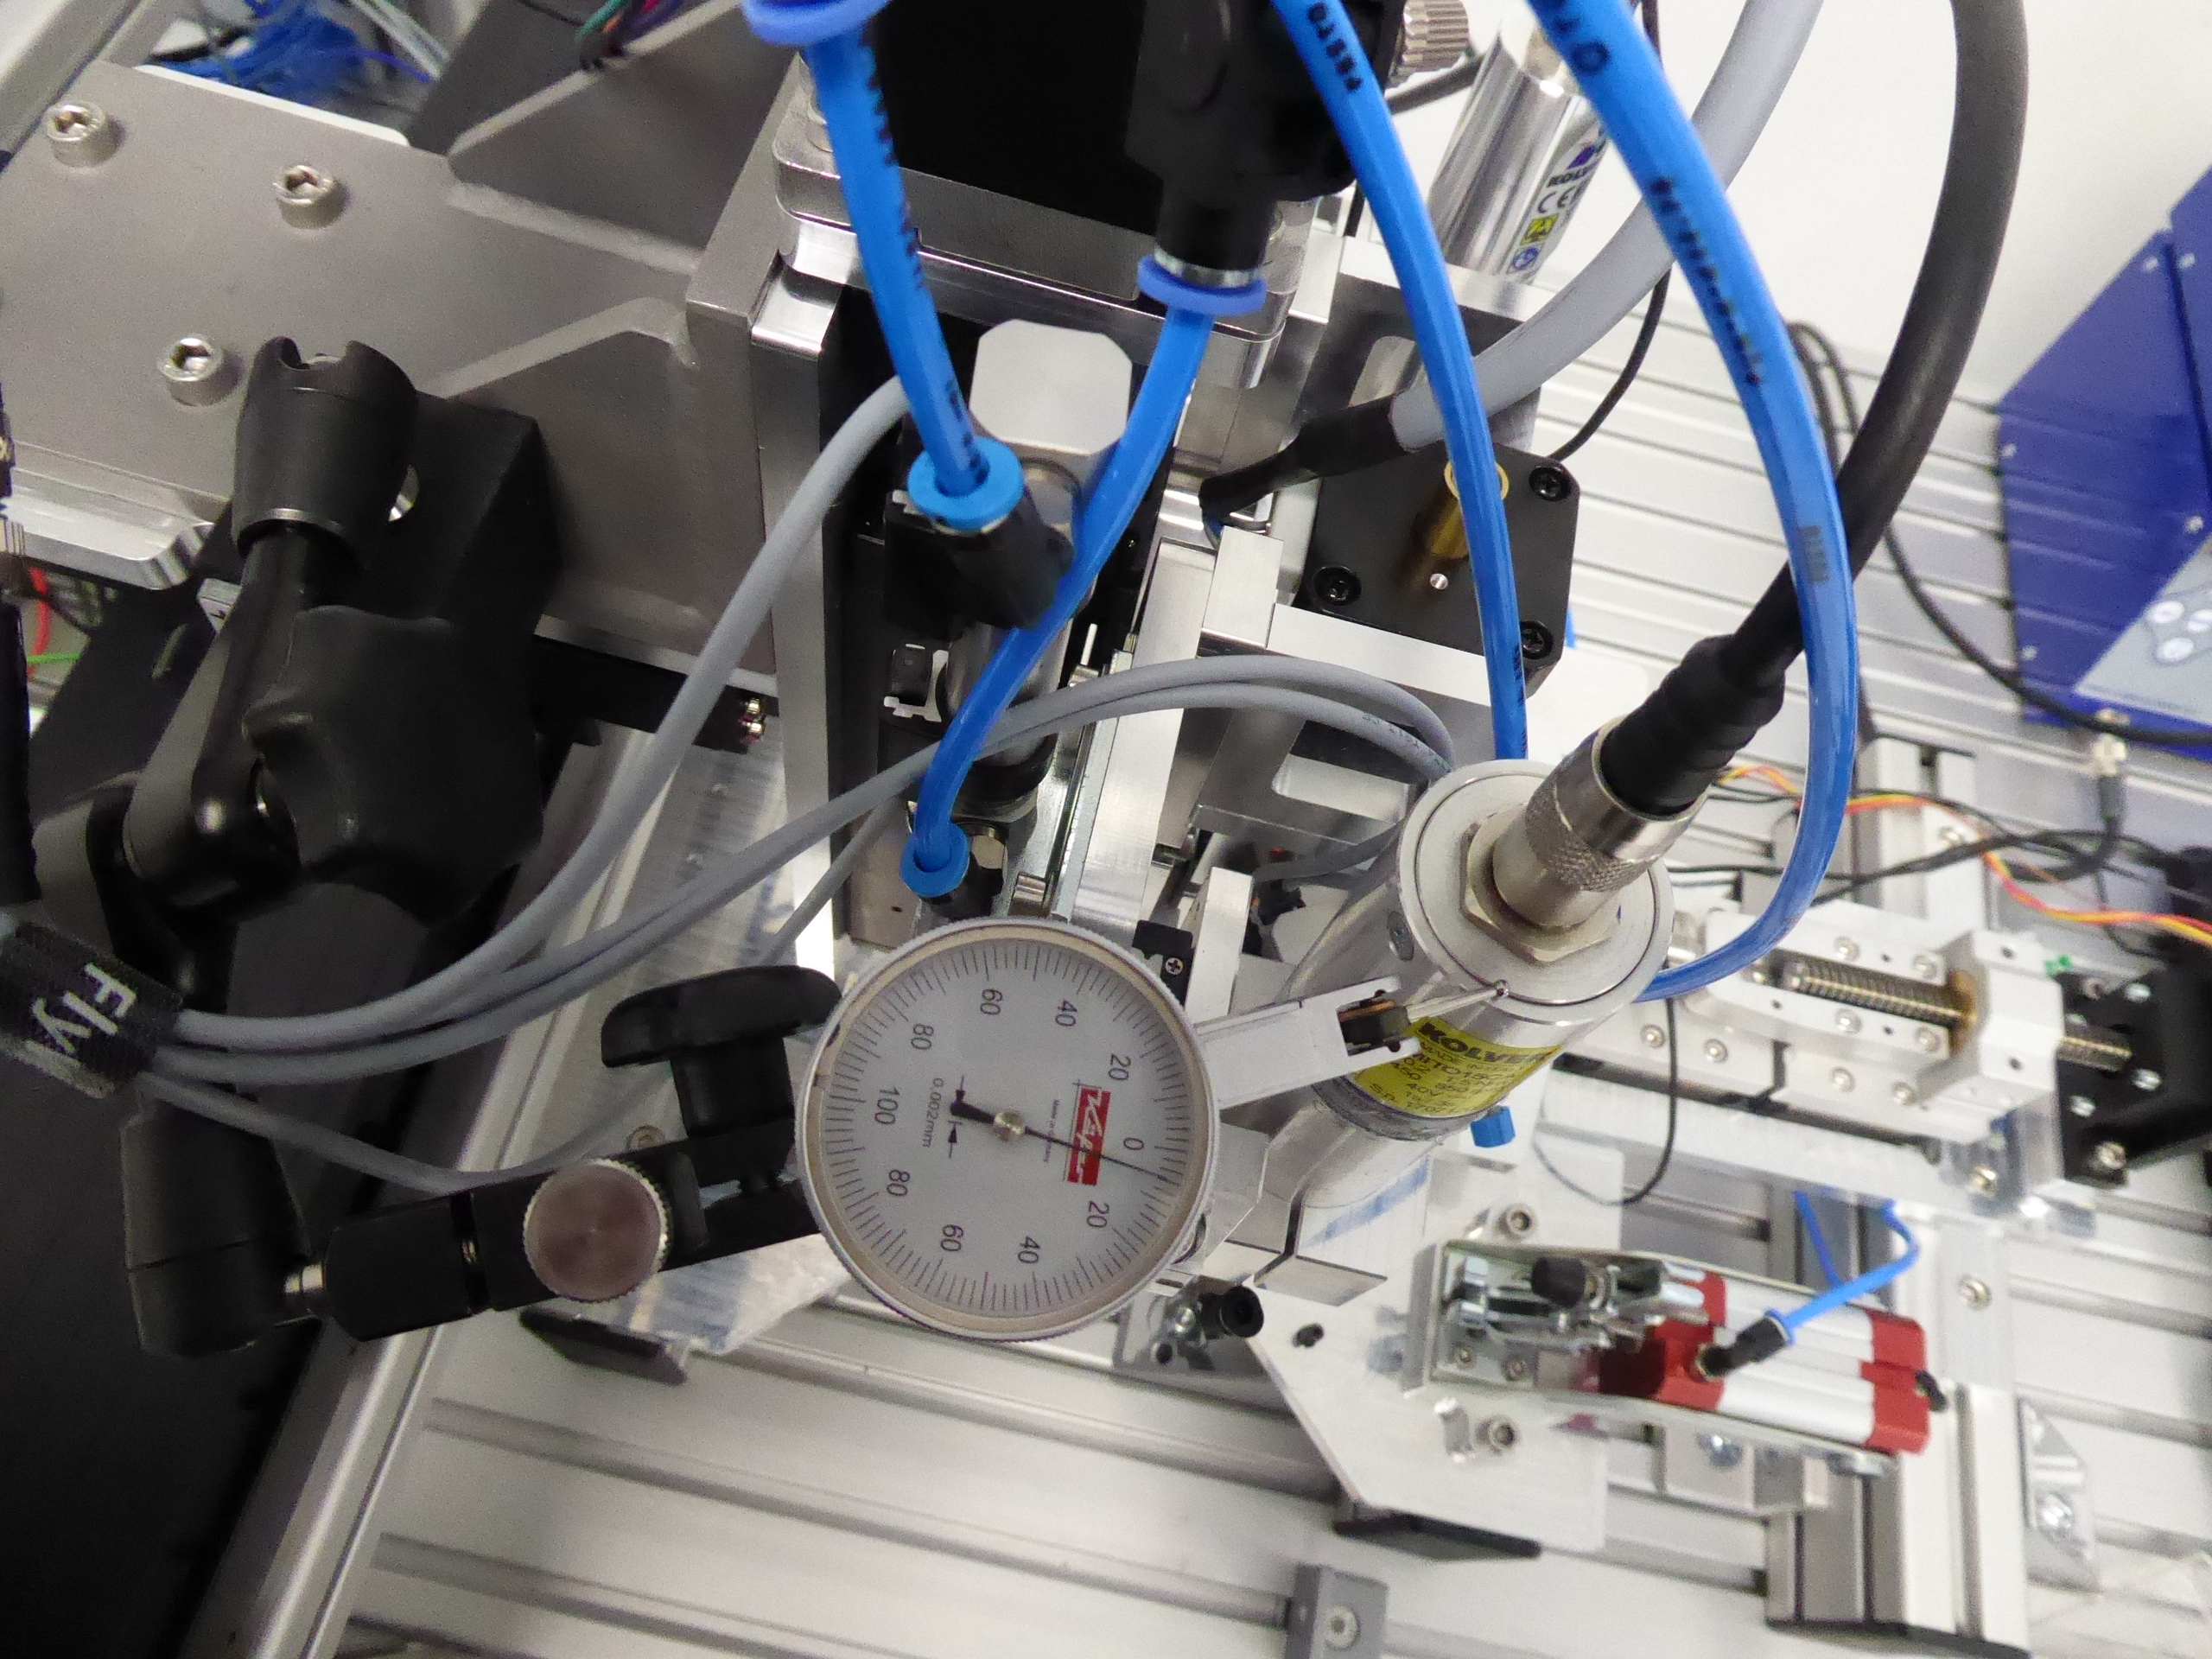
\includegraphics[width=\textwidth]{Bilder/06_Ergebnisse/z_end.JPG}
        \caption{Endposition der Z-Achse}
    \end{subfigure}

    \caption{Messaufbau zur Überprüfung der Wiederholgenauigkeit der Z-Achse}
    \label{fig:z_achse_messung}
\end{figure}

\subsubsection{Tests der Magnetventile und Näherungssensoren}
Die Magnetventile wurden manuell durch Ein- und Ausschalten angesteuert. Dabei wurde überprüft, ob die zugehörigen Näherungssensoren die jeweilige Endlage des Kolbens richtig erfassen. Sowohl die obere als auch die untere Endposition wurden zuverlässig erkannt.

Die Rückmeldungen der Sensoren waren eindeutig und stabil. Damit konnte die korrekte Funktion der Magnetventile in Kombination mit der Endlagensensorik bestätigt werden.

Die Abbildungen~\ref{fig:magnetventil_unten} und~\ref{fig:magnetventil_oben} zeigen die Umschaltung der Näherungssensoren zwischen der unteren und oberen Endlage der Rundkolbenzylinder in Abhängigkeit von der Ventilansteuerung.

\begin{figure}[H]
    \centering
    \begin{subfigure}[t]{0.48\textwidth}
        \centering
        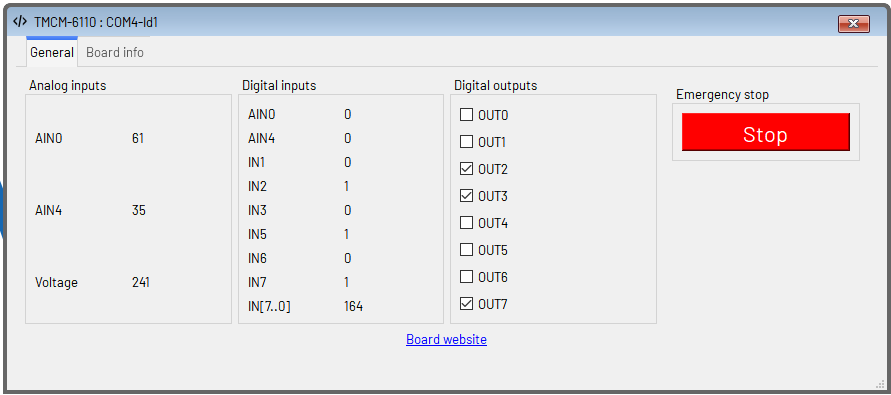
\includegraphics[width=\textwidth]{Bilder/06_Ergebnisse/ventile_an.png}
        \caption{Untere Endlage des Kolbens}
        \label{fig:magnetventil_unten}
    \end{subfigure}
    \hfill
    \begin{subfigure}[t]{0.48\textwidth}
        \centering
        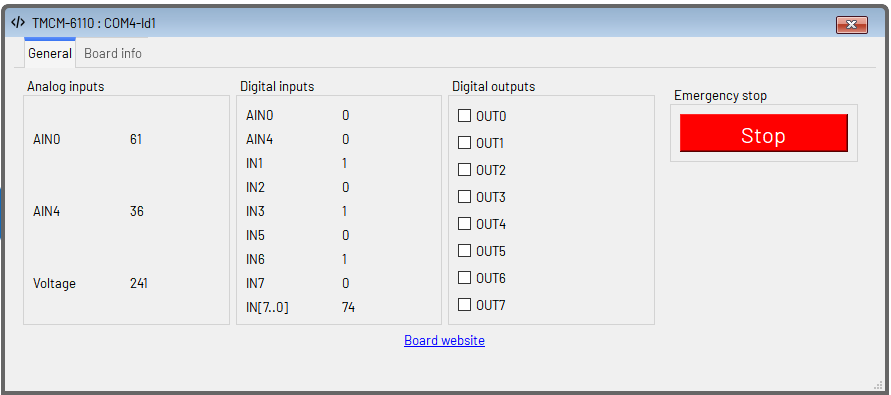
\includegraphics[width=\textwidth]{Bilder/06_Ergebnisse/ventile_aus.png}
        \caption{Obere Endlage des Kolbens}
        \label{fig:magnetventil_oben}
    \end{subfigure}

    \caption{Anzeige der digitalen Ein- und Ausgangssignale während der Ansteuerung der Magnetventile im TMCL-IDE}
    \label{fig:magnetventil_tmcl}
\end{figure}

\subsubsection{Tests der Kraftmessdosen}
Die Kraftmessdosen wurden manuell belastet, um die Signalreaktion zu überprüfen. Die ausgegebenen Messwerte reagierten nachvollziehbar auf Laständerungen und zeigten ein stabiles Verhalten. Die Tara-Funktion arbeitete zuverlässig.

Ein geringes Rauschen war im Signal erkennbar. Da die Kraftmessdosen während der Tests noch nicht vollständig mechanisch fixiert waren, ist dieses Verhalten als unkritisch zu bewerten. Die grundsätzliche Funktionsfähigkeit der Kraftmessdosen konnte bestätigt werden.

Wie in Abbildung~\ref{fig:kmd_rauschen} dargestellt, ist im unbelasteten Zustand der Kraftmessdosen ein geringes Rauschen der Messwerte erkennbar. Dieses Verhalten ist auf den noch nicht vollständig fixierten mechanischen Aufbau während der Tests zurückzuführen und wird als unkritisch bewertet.

Bei manueller Belastung der Kraftmessdosen zeigen die Messwerte eine eindeutige und reproduzierbare Änderung, wie in den Abbildungen~\ref{fig:kmd_belastet_1} und~\ref{fig:kmd_belastet_2} zu sehen ist. Der jeweilige Belastungszustand wird zusätzlich über die digitalen Eingänge korrekt signalisiert, wodurch die Funktion der Kraftmessdosen bestätigt werden kann.

\begin{figure}[H]
    \centering
    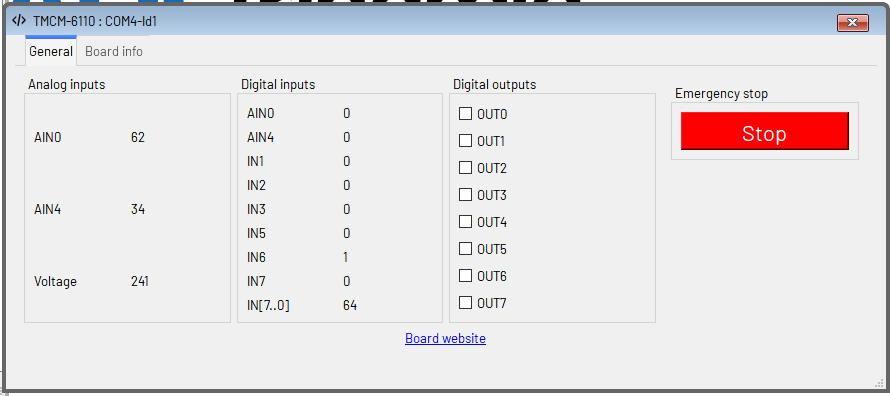
\includegraphics[width=0.7\textwidth]{Bilder/06_Ergebnisse/kmd_unbelastet.png}
    \caption{Messwertanzeige der Kraftmessdosen im unbelasteten Zustand mit erkennbaren Rauschanteilen}
    \label{fig:kmd_rauschen}
\end{figure}

\begin{figure}[H]
    \centering
    \begin{subfigure}[t]{0.48\textwidth}
        \centering
        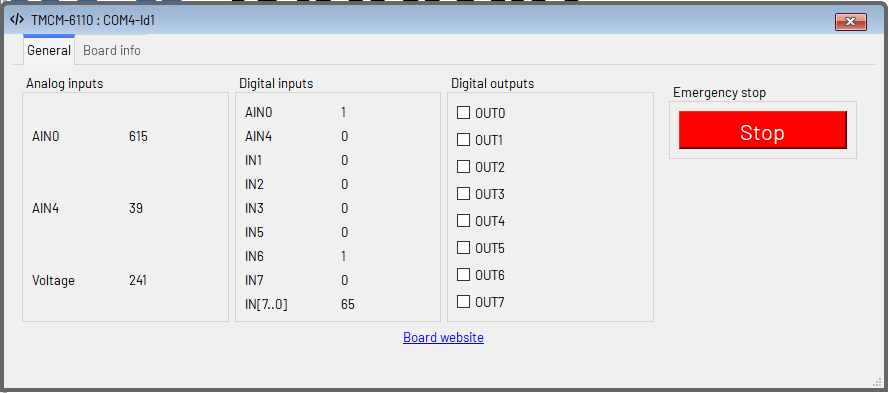
\includegraphics[width=\textwidth]{Bilder/06_Ergebnisse/kmd_vorspann.png}
        \caption{Manuelle Belastung der Kraftmessdose im Vorspannsystem}
        \label{fig:kmd_belastet_1}
    \end{subfigure}
    \hfill
    \begin{subfigure}[t]{0.48\textwidth}
        \centering
        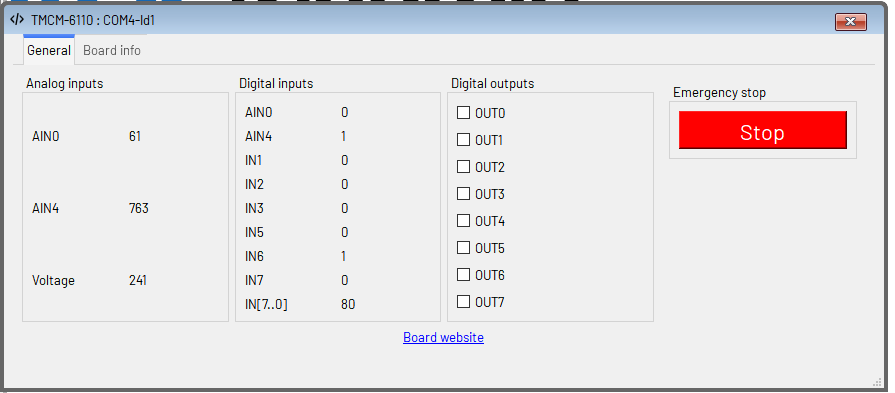
\includegraphics[width=\textwidth]{Bilder/06_Ergebnisse/kmd_keile.png}
        \caption{Manuelle Belastung der Kraftmessdose im Keile-Einpresssystem}
        \label{fig:kmd_belastet_2}
    \end{subfigure}

    \caption{Messwertänderung der Kraftmessdosen bei manueller Belastung mit zugehöriger digitaler Rückmeldung}
    \label{fig:kmd_belastet}
\end{figure}


\subsection{Durchgeführte Tests mit der WAGO-Steuerung}
\subsubsection{Tests der Laser-Triangulation Sensor}
Zur Überprüfung des Laser-Triangulationssensors wurde der Schlitten entlang der Messachse verfahren und der erfasste Abstand mit einer manuellen Referenzmessung verglichen. Die vom Sensor ausgegebenen Messwerte erwiesen sich als plausibel und reproduzierbar.

Die durchgeführten Tests zeigen, dass der Sensor zuverlässig arbeitet und für die Positions- und Abstandsüberwachung innerhalb des Systems geeignet ist.

\begin{figure}[H]
    \centering
    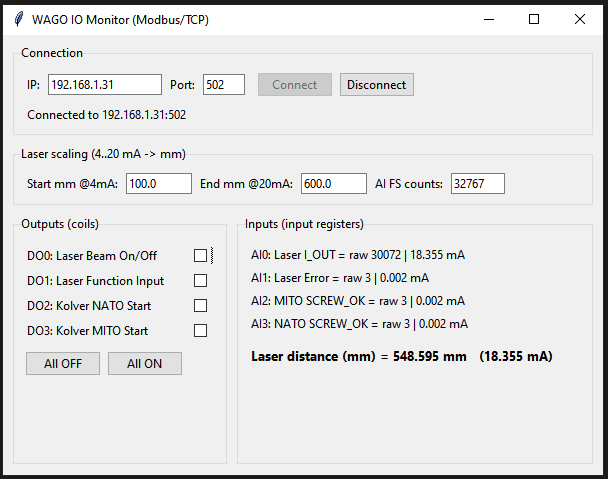
\includegraphics[width=0.85\textwidth]{Bilder/06_Ergebnisse/laser_distance.png}
    \caption{Ausgabe der Messwerte des Laser-Triangulationssensors im WAGO IO Monitor während der Verfahrbewegung des Schlittens}
    \label{fig:laser_wago}
\end{figure}

\subsubsection{Tests der automatische Schraubendreher}
Die automatischen Schraubendreher wurden hinsichtlich der Ansteuerung und Rückmeldung getestet. Start-, Stopp- und Statussignale wurden korrekt auf der Anzeige des EDU-Systems dargestellt. Auch Fehlversuche wurden zuverlässig angezeigt.

Bei Tests ohne eingesetzte Schraube zeigte sich, dass das Signal „Screw OK“ kurzzeitig auf den Wert~1 gesetzt wurde und anschließend wieder auf~0 zurückfiel. Dieses Verhalten trat ausschließlich bei Leerlauftests auf und ist auf den fehlenden realen Schraubprozess zurückzuführen.

\begin{figure}[H]
    \centering
    \begin{subfigure}[t]{0.32\textwidth}
        \centering
        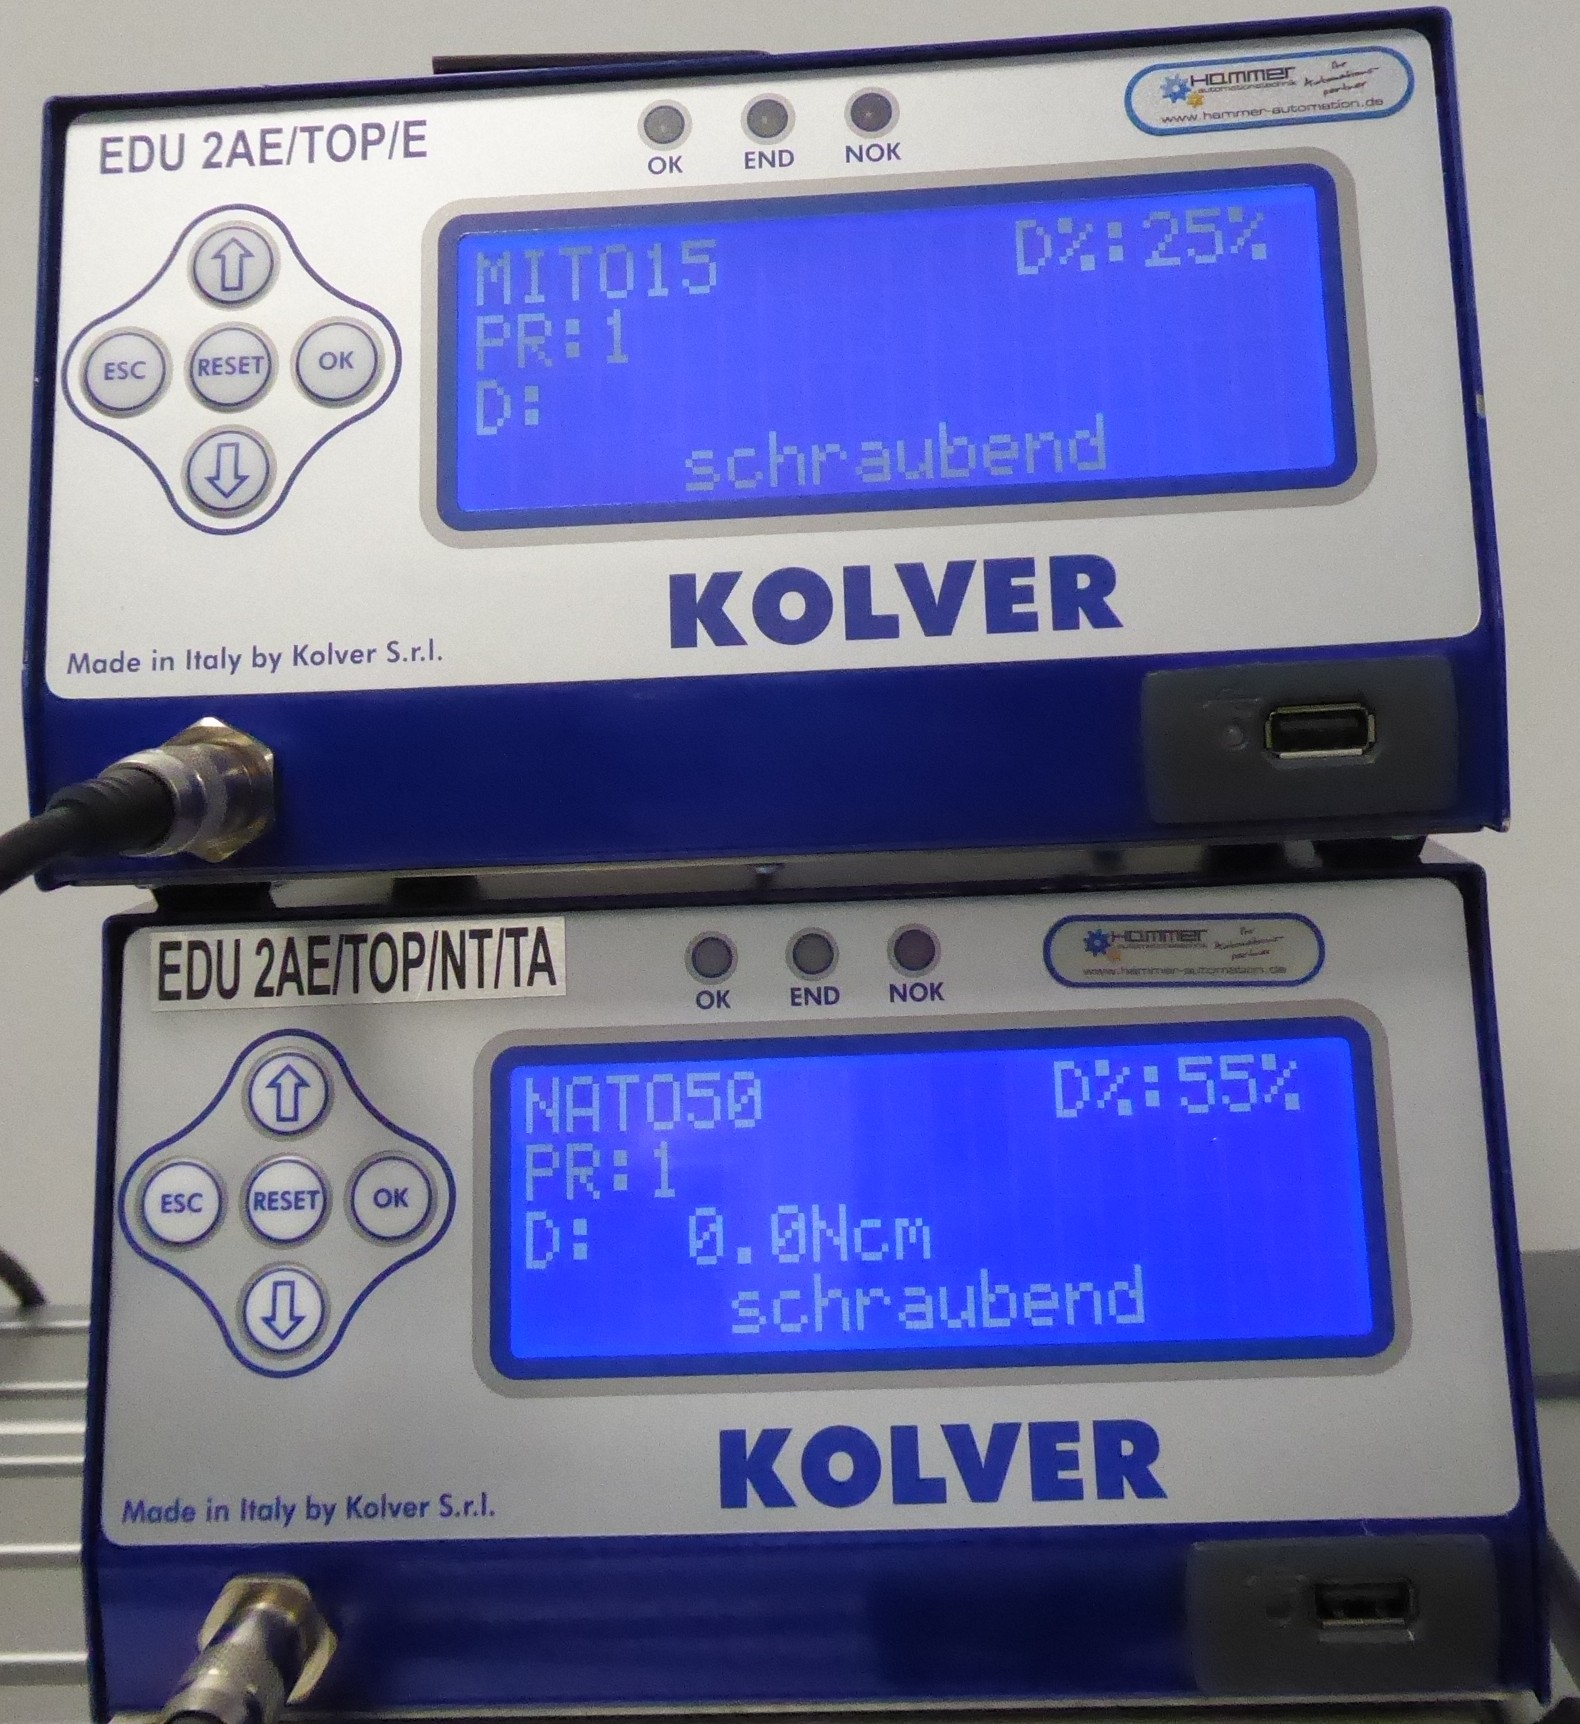
\includegraphics[width=\textwidth]{Bilder/06_Ergebnisse/kolver_init.JPG}
        \caption{Initialzustand der EDU-Anzeige}
        \label{fig:kolver_init}
    \end{subfigure}
    \hfill
    \begin{subfigure}[t]{0.32\textwidth}
        \centering
        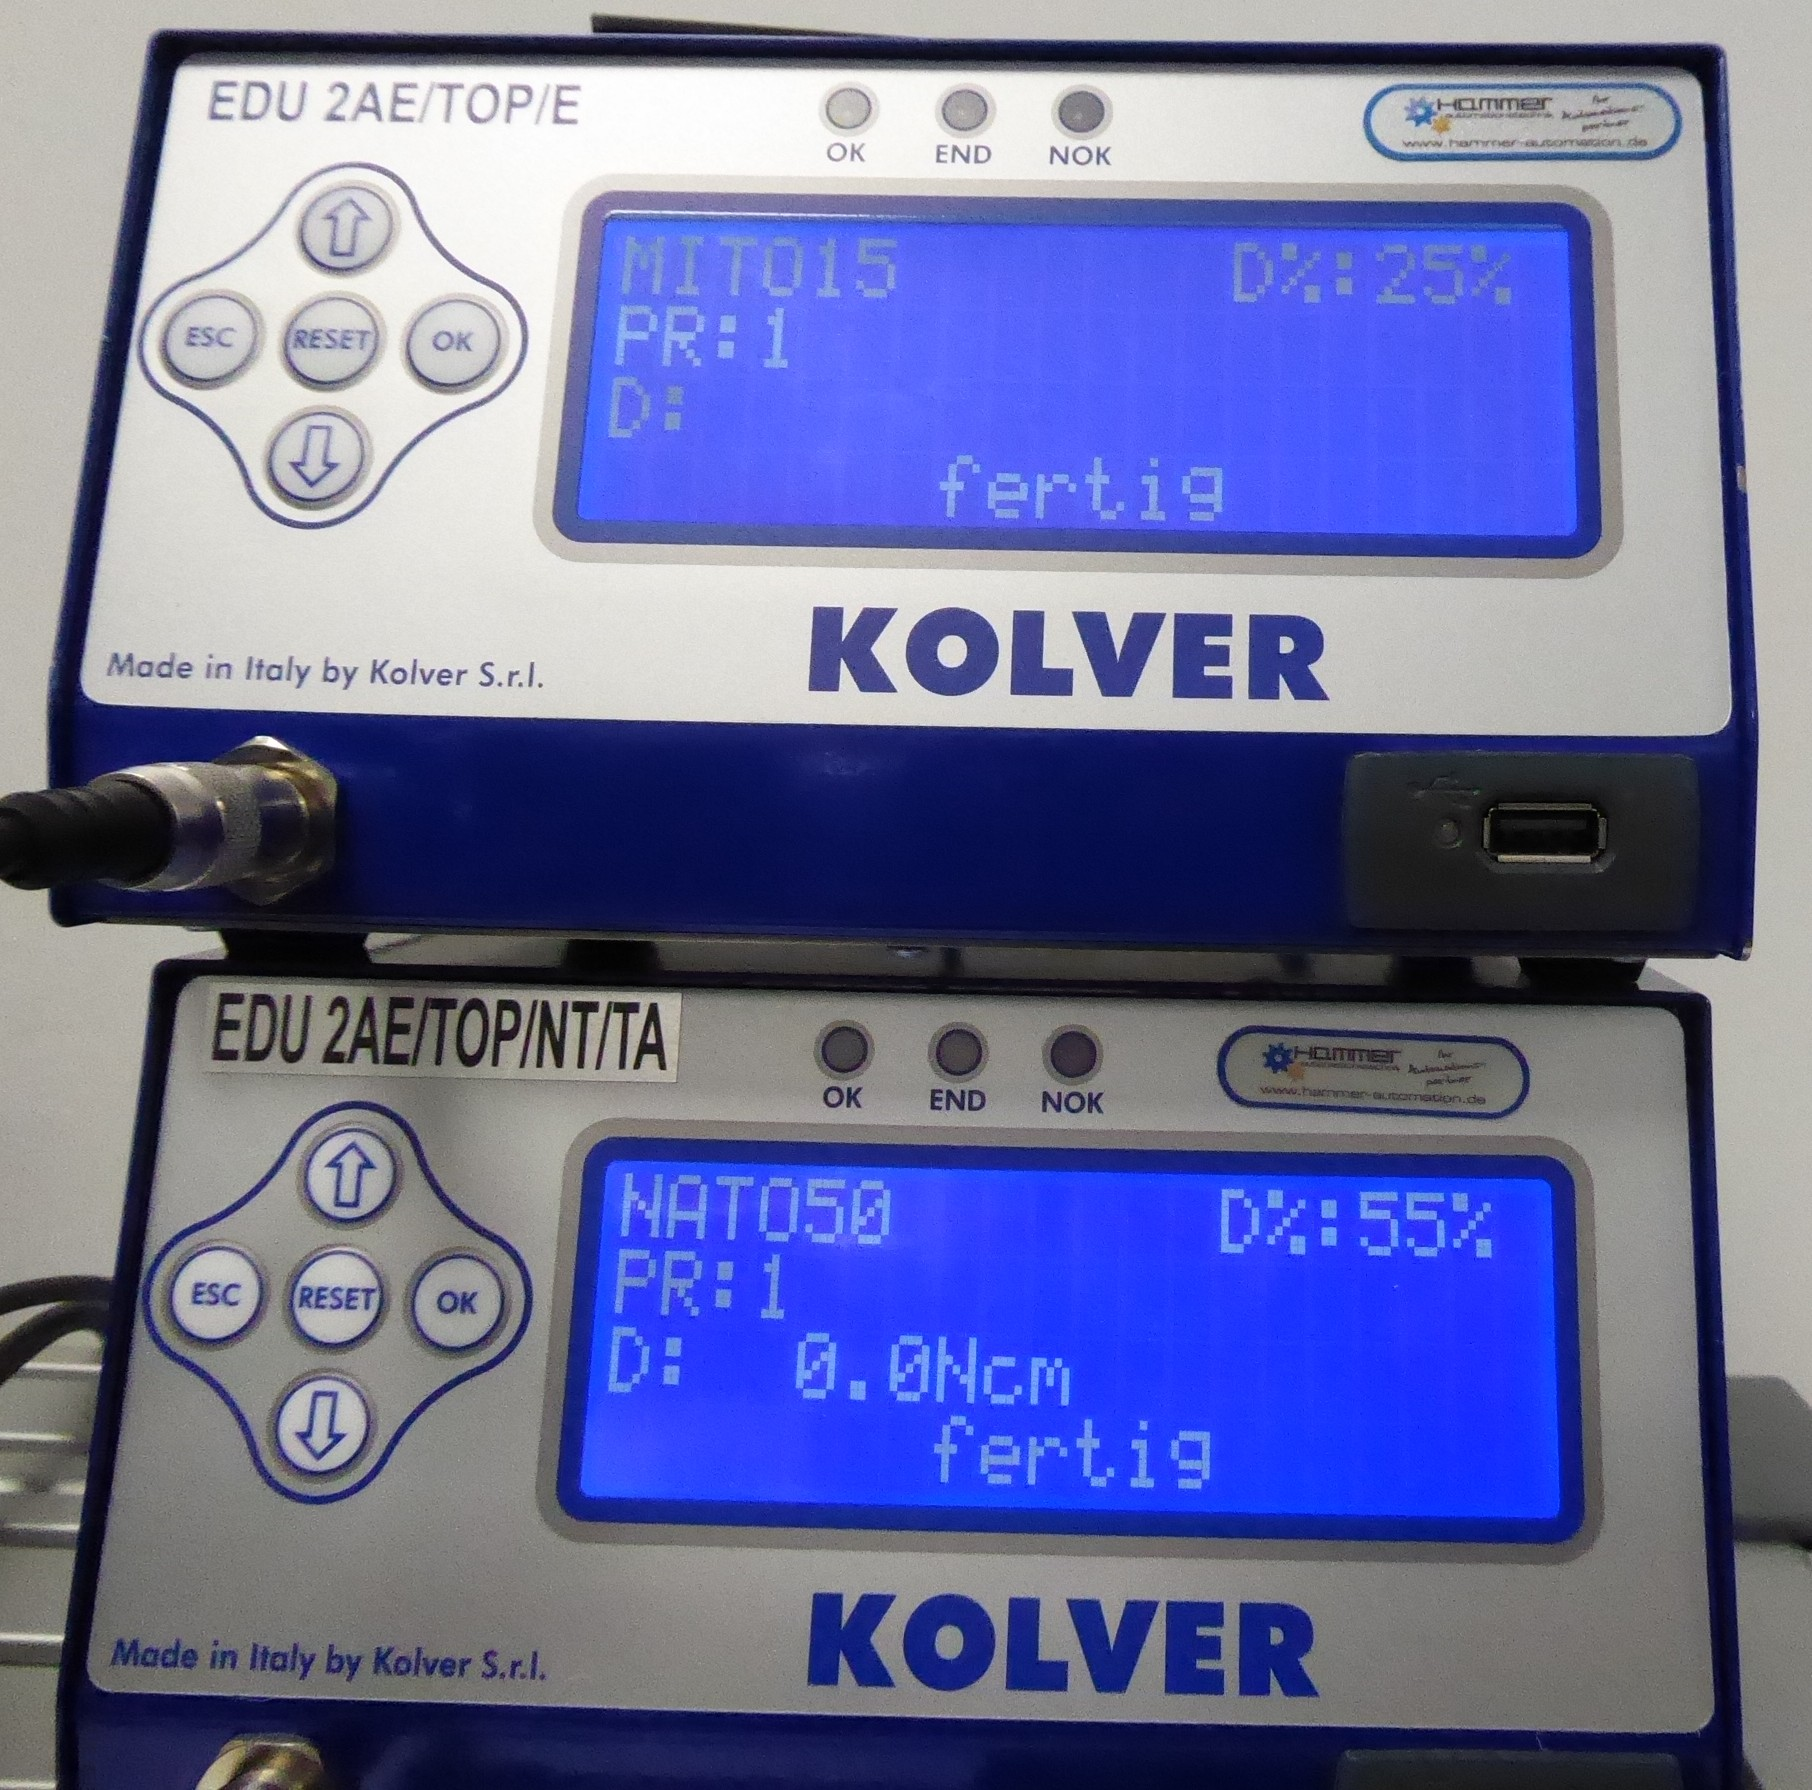
\includegraphics[width=\textwidth]{Bilder/06_Ergebnisse/kolver_ok.JPG}
        \caption{Erfolgreicher Verschrauben}
        \label{fig:kolver_ok}
    \end{subfigure}
    \hfill
    \begin{subfigure}[t]{0.32\textwidth}
        \centering
        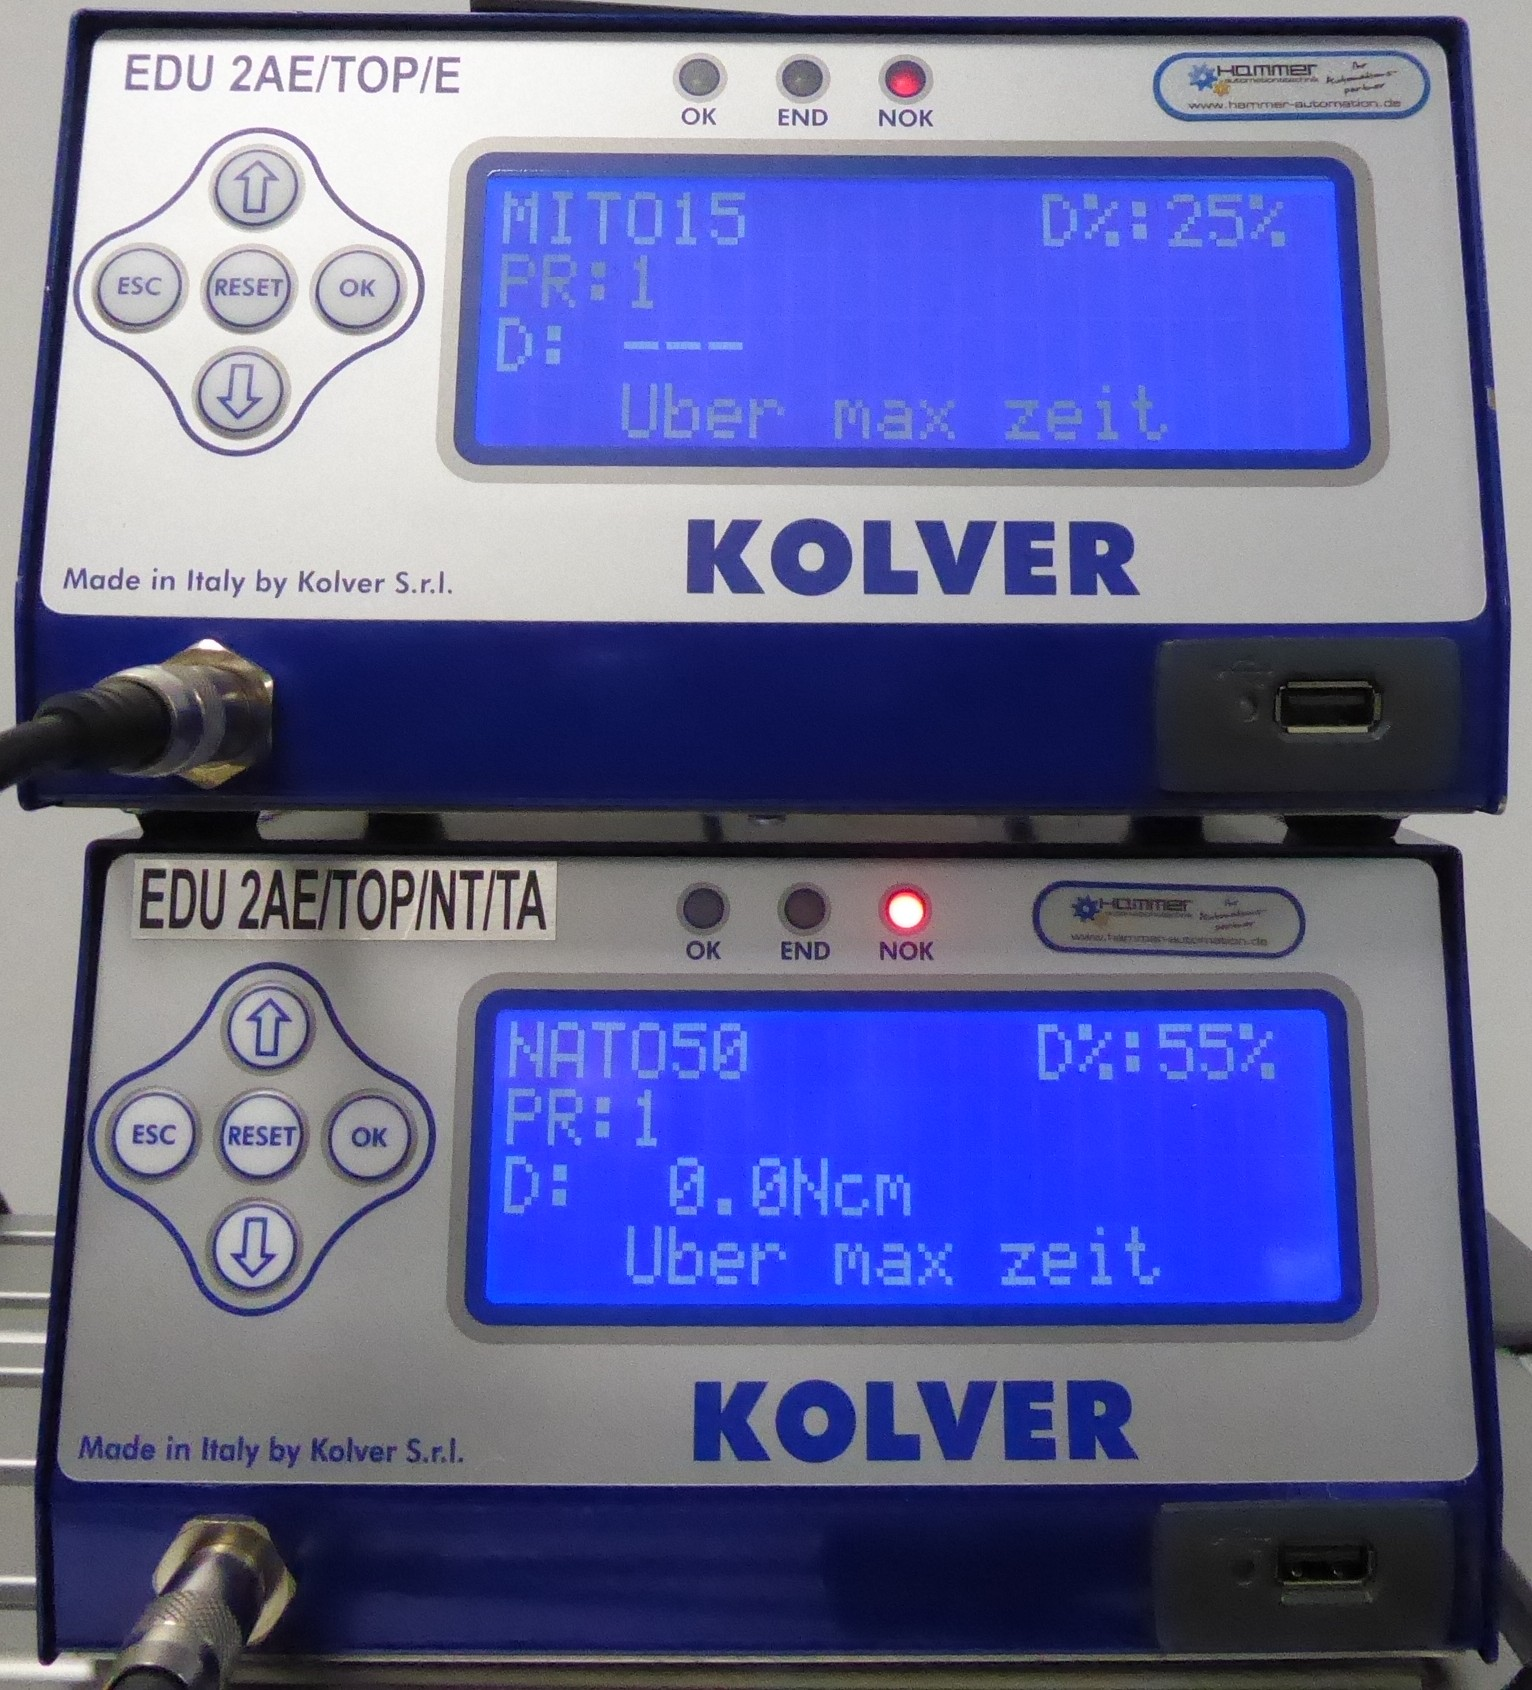
\includegraphics[width=\textwidth]{Bilder/06_Ergebnisse/kolver_nok.JPG}
        \caption{Fehlversuch bei Leerlauftest}
        \label{fig:kolver_nok}
    \end{subfigure}

    \caption{Anzeigezustände der automatischen Schraubendreher auf der EDU-Anzeige während der Tests}
    \label{fig:kolver_zustaende}
\end{figure}

\subsection{Messergebnisse und Beobachtungen}
Die Validierungstests zeigen, dass alle getesteten Aktoren und Sensoren wie vorgesehen funktionieren. Die Positioniergenauigkeit der Linearachsen liegt innerhalb der definierten Toleranzen, und die Sensorik liefert stabile und nachvollziehbare Messwerte.

Es traten keine grundlegenden Probleme auf. Einzelne Auffälligkeiten sind auf den vereinfachten Testaufbau und den Prototypenstatus des Systems zurückzuführen. Für eine abschließende Bewertung wären weiterführende Tests im vollständig integrierten Aufbau erforderlich.

Insgesamt bestätigen die Ergebnisse die grundsätzliche Eignung des entwickelten Systems für den vorgesehenen Montageprozess.\cite{man_trinamic_tmcm6110,man_wago_750system,ds_microepsilon_optoncdt1220}
